\chapter{Ejecución de las simulaciones}
\label{ch:simulations}
\lhead{\emph{Ejecución de las simulaciones}}

\todo{Cosas a terminar al volver a correr el programa:
* Especificar que se acepta una mascara de +- 1dB}

En este capítulo se presentan los casos de simulación, que se construyen sobre la base del modelo de antena desarrollado para
estudiar y comparar como se comportan ambos métodos de calibración interna: clásica y complementaria utilizando acoplamientos
mutos entre polarizaciones ortogonales.

En las secciones listadas a continuación se simulan todos los posibles casos de error individualmente.
\begin{enumerate}
	\item En la sección \ref{sc:withoutDispersion} se simula el comportamiento de ambos calibradores con la antena sin
		dispersiones de ningún tipo.
	\item En la sección \ref{sc:trmsDamaged} se simula el comportamiento de ambos calibradores con dos TRMs dañados, o muertos.
	\item En la sección \ref{sc:withDispersion} se simula el comportamiento de ambos calibradores con dispersiones en los
		componentes internos de la antena.
	\item En la sección \ref{sc:withPulsesGainDispersion} se simula el comportamiento de ambos calibradores con dispersiones en
		la potencia y fase de la señal de calibración.
	\item En la sección \ref{sc:withChirpPulsesGainDispersion} se simula el comportamiento del calibrador clásico con 
		dispersiones en la chirp réplica. 
	\item En la sección \ref{sc:withWalshDispersion} se simula el comportamiento del calibrador clásico con dispersiones en las
		configuraciones de fase de los TRMs en la codificación de los códigos Walsh.
\end{enumerate}

A su vez, en la sección \ref{sc:montecarlo} se realiza un montecarlo de 1000 realizaciones simulando el comportamiento de ambos
calibradores con todos los posibles errores. 

Por último, en la sección \ref{sc:relationDispersionRadiationPattern} se realiza un estudio de la relación entre el desvío en
ganancia del lóbulo principal del diagrama de radiación en función del desvío de la ganancia y fase emitida por cada ER.


\section{Características de ensayos y presentación de resultados}
\label{sc:characteristics}

Todos los casos de simulación realizados con ambos calibradores en las secciones previamente mencionadas poseen las siguientes
características:
\begin{enumerate}
	\item Se calibra con tres apuntamientos distintos. Los cuales son uniforme (implica que todos los TRMs desfasan cero grados),
		10 grados en la dirección horizontal, o azimut, y 10 grados en la dirección vertical, o rango. Se proponen distintos de
		apuntamientos para evaluar cómo funcionan los métodos. 
	\item Se muestran dos gráficos, de potencia y fase transmitida por cada ER para cada apuntamiento utilizado. En los cuales se
		observan las señales sin calibrar, la cual se corresponde a la señales previa a la calibración, calibrada e ideal. 
	\item Se grafican los diagramas de radiación de la antena para los cortes horizontal y vertical de las señales transmitidas
		sin calibrar, calibradas e ideales.
	\item Para una mayor claridad en los gráficos, se presentan los resultados de las calibraciones para un estado puntual, en
		otras palabras, no se realizan ensayos de montecarlo. Salvo que dentro de la sección se indique lo contrario.
\end{enumerate}


\section{Configuración de antena}

La configuración de la antena a utilizar para todos los casos de simulación está especificada en el cuadro
\ref{tab:configurationUsed} y consta de 70 elementos radiantes. Las especificaciones de las propiedades físicas de cada
componente están definidas en la tabla \ref{tab:configurationOfComponents}.
\begin{table}[H]
  \footnotesize
  \centering
  \begin{tabular}{|c|c|}
	\hline
	\textbf{Componente de Antena} & \textbf{Configuración} \tabularnewline \hline 
	freq &  1.275 [MHz] \tabularnewline\hline 
	power & 0 [dB] \tabularnewline \hline 
	phase & 0 [deg] \tabularnewline \hline 
	desiredTxPower & 6 [dB] \tabularnewline \hline 
	desiredRxPower & 0 [dB] \tabularnewline \hline 
	quantityRows & 7 \tabularnewline \hline 
	quantityColumns & 10 \tabularnewline \hline 
	verticalSeparation & 0.2 [m] \tabularnewline \hline 
	horizontalSeparation & 0.2 [m] \tabularnewline \hline 
	componentSequence & [cable1, psc17, cable1, psc15, cable2, psc12, trm, circulator, cable3, rm] \tabularnewline \hline 
  \end{tabular}
  \caption{Configuración de la antena común para todos los casos de simulación.}
  \label{tab:configurationUsed}
\end{table}
\begin{table}[H]
  \footnotesize
  \centering
  \begin{tabular}{|c|c|c|}
	\hline
	\textbf{Componente de Antena} & \textbf{Características físicas} & \textbf{Configuración} \tabularnewline \hline 
	\multirow{2}{*}{cable1} &  attenuation [db] & 0.1\tabularnewline \cline{2-3}
	 & length [m] & 0.45\tabularnewline \hline 
	\multirow{2}{*}{cable2} &  attenuation [db] & 0.1\tabularnewline \cline{2-3}
	 & length [m] & 8\tabularnewline \hline 
	\multirow{2}{*}{cable3} &  attenuation [db] & 0.1\tabularnewline \cline{2-3}
	 & length [m] & 0.5\tabularnewline \hline 
	psc17 & outputPorts & 7\tabularnewline \hline
	psc15 & outputPorts & 5\tabularnewline \hline
	psc12 & outputPorts & 2\tabularnewline \hline
	\multirow{2}{*}{TRM} & gain [db] & 10\tabularnewline \cline{2-3}
	 & phaseShift [deg] & 10\tabularnewline \hline 
	circulator & & \tabularnewline \hline 
	RM & & \tabularnewline \hline 
  \end{tabular}
  \caption{Configuración de las propiedades físicas de cada componente de la antena utilizada en todos los casos de simulación.}
  \label{tab:configurationOfComponents}
\end{table}

Exceptuando la cantidad de elementos radiantes, el resto de las configuraciones fueron definidas de forma arbitraria. La
elección de los 70 elementos radiantes fue realizada por los siguientes motivos:
\begin{itemize}
	\item Si bien la cantidad de elementos radiantes son pocos para una antena, los resultados no dejan de ser representativos.
	\item Si se elige una mayor cantidad de ER el programa tarda más en procesar. 
	\item Los valores de ganancia y fase individual de cada ER estarían más solapados entre sí, haciendo que no se pueda apreciar
		cada resultado individualmente. 
	\item En el desarrollo teórico se llegó a la conclusión que el método solamente tiene una cota inferior en la cantidad de ER
		para la viabilidad de su uso dado que al agregar más ER se introducen más posibles lazos de calibración que ecuaciones.
\end{itemize}

La numeración de los elementos radiantes tiene un orden creciente de izquierda a derecha y de arriba hacia abajo, de tal forma
que el elemento cero es el superior izquierdo de la antena, la figura \ref{fig:arrayNumeration} representa un ejemplo.

\begin{figure}[H]
 \centering
 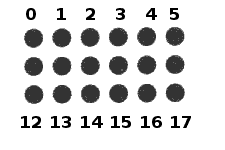
\includegraphics[width=7cm]{gfx/arrayNumeration.png}
 \caption{Numeración de los elementos de un panel de antena.}
 \label{fig:arrayNumeration}
\end{figure}


\section{Caso ideal}
\label{sc:withoutDispersion} 

Los casos de simulación de esta sección presenta una antena con las siguientes características,
\begin{itemize}
	\item Los componentes de antena funcionan normalmente, son ideales.
	\item No hay dispersiones en la señal, la misma es invariante en el tiempo.
\end{itemize}


\subsection{Calibración interna clásica en el caso ideal}

A continuación se presentan los tres casos de prueba definidos en la sección \ref{sc:characteristics} para el método de
calibración interna clásico.

\subsubsection{Apuntamiento uniforme}

Los gráficos de la figura \ref{fig:nonErrClassical0deg} muestran que el calibrador, por no abarcar la totalidad del sistema, no 
puede determinar correctamente ni la ganancia ni fase de la antena. Aun así, como dicho desvío es el mismo para todos los
elementos el diagrama de radiación resultante mantiene su forma y sus atributos no se modifican, salvo la ganancia total. A su
vez, se observa que la ganancia y fase es la misma en todos los elementos de la antena, por ello se le da el nombre de uniforme.
De los diagramas de radiación se ve el máximo en el centro (cero grados de inclinación de apuntamiento) y se observan los
lóbulos secundarios a 12.97 dBc por debajo del lóbulo primario.

Los tres estados de señales graficados son el deseado (caso ideal), el previo a calibrar (non-cal) y el resultante de la
calibración (cal).

\begin{figure}[H]
	\centering
 	\subfloat[Ganancia y fase transmitida por cada ER]{
		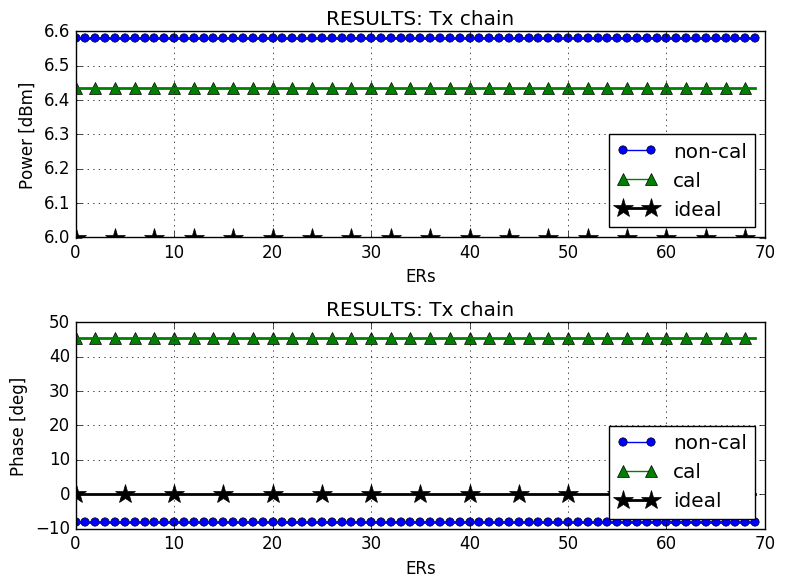
\includegraphics[width=9cm]{gfx/nonErrClassical0deg.png}}

	\subfloat[Corte en azimut (horizontal) del diagrama de radiación]{
		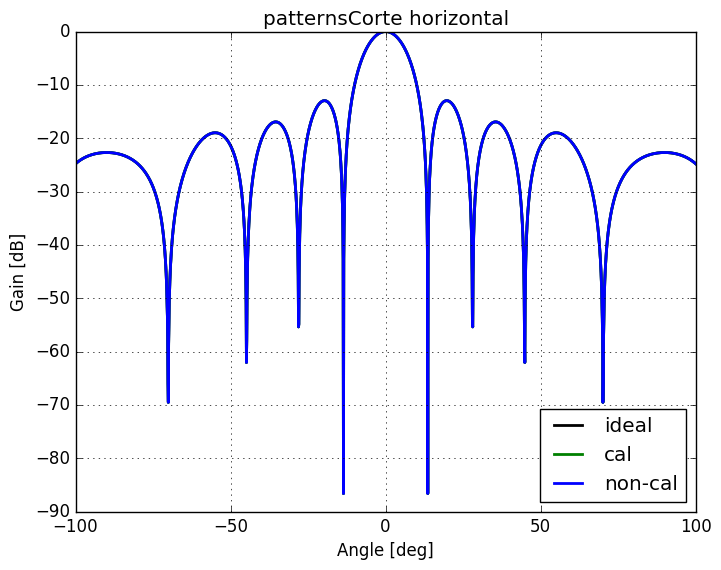
\includegraphics[width=7cm]{gfx/nonErrClassical0degAzCut.png}}
	\subfloat[Corte en rango (vertical) del diagrama de radiación]{
		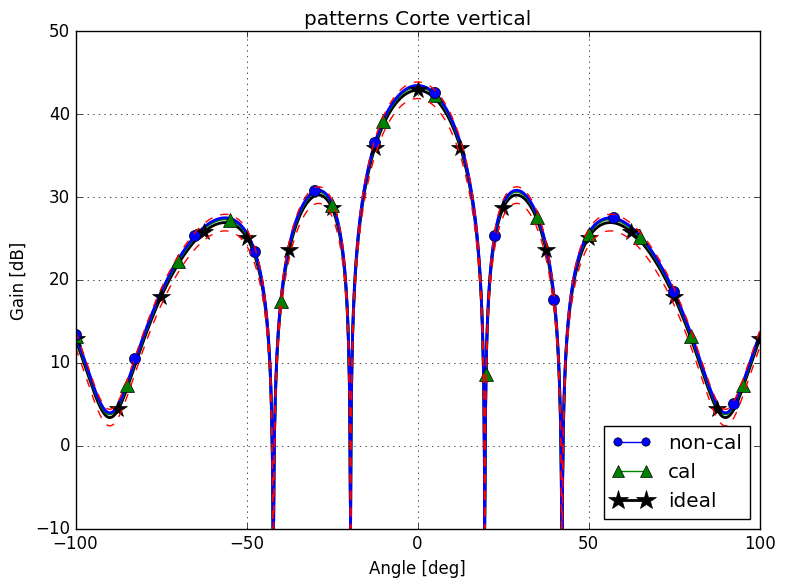
\includegraphics[width=7cm]{gfx/nonErrClassical0degElCut.png}}
		\caption{Señales transmitidas por la antena en los casos deseado (ideal), pre (non-cal) y post (cal) calibración clásica.}
	\label{fig:nonErrClassical0deg}
\end{figure}

La tabla \ref{tab:nonErrClassical0deg} muestra como la ganancia relativa de los lóbulos secundarios con respecto al del lóbulo
principal de cada diagrama se mantienen invariantes e iguales al del diagrama ideal, 12.97 dBc en polarización H y 12.65 dBc en
polarización V. A su vez se puede observar que, dado que el esquema de calibración no abarca la totalidad del sistema, la
diferencia de la ganancia del diagrama calibrado disminuye pero no llega a ser igual a cero.

\begin{table}[H]
  \footnotesize
  \centering
  \begin{tabular}{|c|c|C{2cm}|C{2.5cm}|C{2.5cm}|C{2.5cm}|}
    \hline
    Caso & Corte & Ganancia - lóbulo izq. [dBc] & Ganancia - lóbulo central [dB] &
    Ganancia - lóbulo der. [dBc] & Ancho - lóbulo central -3dB \tabularnewline\hline
    \multirow{2}{2cm}{Diag. rad. sin calibrar} & H & 12.97 & 43.48 & 12.97 & 12.0 \tabularnewline\cline{2-6}
     & V & 12.65 & 43.48 & 12.65 & 17.4 \tabularnewline\hline
    \multirow{2}{2cm}{Diag. rad. calibrado} & H & 12.97 & 43.34 & 12.97 & 12.0 \tabularnewline\cline{2-6}
     & V & 12.65 & 43.34 & 12.65 & 17.4 \tabularnewline\hline
    \multirow{2}{2cm}{Diag. rad. ideal} & H & 12.97 & 42.9 & 12.97 & 12.0 \tabularnewline\cline{2-6}
     & V & 12.65 & 42.9 & 12.65 & 17.4 \tabularnewline\hline
    \multirow{2}{2cm}{Dif. sin calibrar} & H & 0.0 & 0.58 & 0.0 & 0.0\tabularnewline\cline{2-6}
     & V & 0.0 & 0.58 & 0.0 & 0.0 \tabularnewline\hline
    \multirow{2}{2cm}{Dif. calibrado} & H & 0.0 & 0.44 & 0.0 & 0.0 \tabularnewline\cline{2-6}
     & V & 0.0 & 0.44 & 0.0 & 0.0 \tabularnewline\hline
  \end{tabular}
  \caption{Propiedades de los diagramas de radiación calibrados y sin calibrar comparados con el ideal.}
  \label{tab:nonErrClassical0deg}
\end{table}


\subsubsection{Apuntamiento 10 grados en azimut (horizontal)}

Los gráficos de la figura \ref{fig:nonErrClassical10degCol} muestran que el calibrador, por no abarcar la totalidad del sistema, no 
puede determinar correctamente ni la ganancia ni fase de la antena. Aun asi, como dicho desvío es el mismo para todos los
elementos el diagrama de radiación resultante mantiene su forma y sus atributos no se modifican, salvo la ganancia total.

Se observa que la ganancia es la misma en todos los elementos de antena, pero que la fase presenta una distribución diente de
sierra porque se está apuntado horizontalmente, por ende, todos los elementos que pertenecen a un mismo panel, o columna, poseen
la misma fase y entre paneles hay un desfase lineal porque la separación es uniforme. Por ejemplo, los ER número 3, 13, 23, 33,
43, 53 y 63, pertenecientes al segundo panel, poseen una fase ideal aproximada a los -50 grados.

El desfase entre paneles depende de la inclinación del frente de onda deseado, la frecuencia de la señal utilizada y de la
separación entre elementos radiantes.

De los diagramas de radiación se observa el máximo en los diez grados para el corte horizontal y en cero grados para el corte
vertical y que los lóbulos secundarios se encuentran aproximadamente a 13 dBc por debajo de dichos máximos.

Los tres estados de señales graficados son el deseado (caso ideal), el previo a calibrar (non-cal) y el resultante de la
calibración (cal).

\begin{figure}[H]
	\centering
 	\subfloat[Ganancia y fase transmitida por cada ER]{
		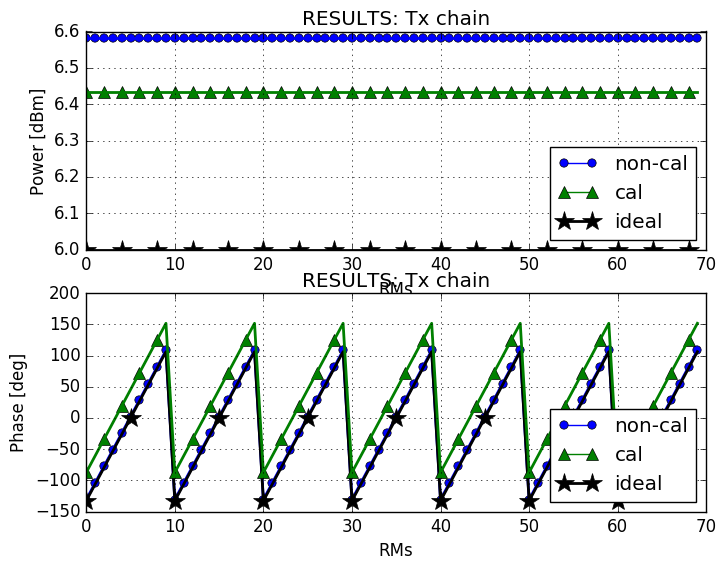
\includegraphics[width=9cm]{gfx/nonErrClassical10degCol.png}}

	\subfloat[Corte en azimut (horizontal) del diagrama de radiación]{
		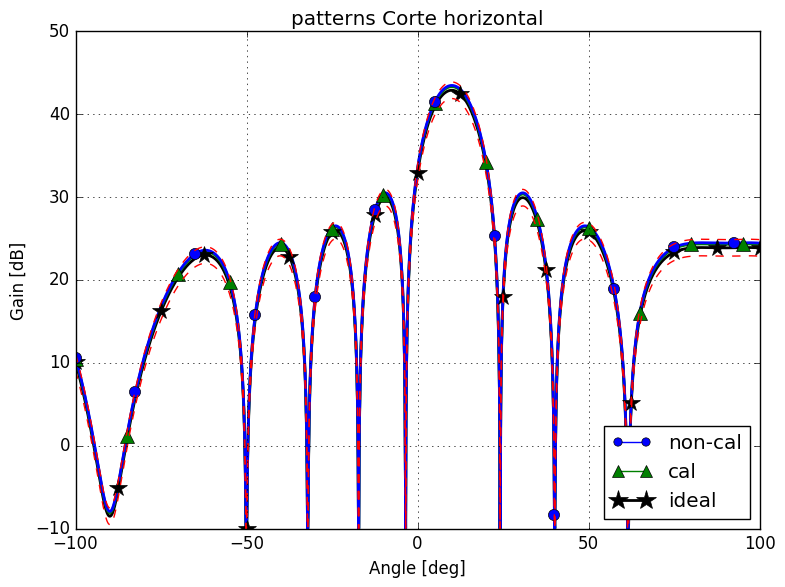
\includegraphics[width=7cm]{gfx/nonErrClassical10degColAzCut.png}}
	\subfloat[Corte en rango (vertical) del diagrama de radiación]{
		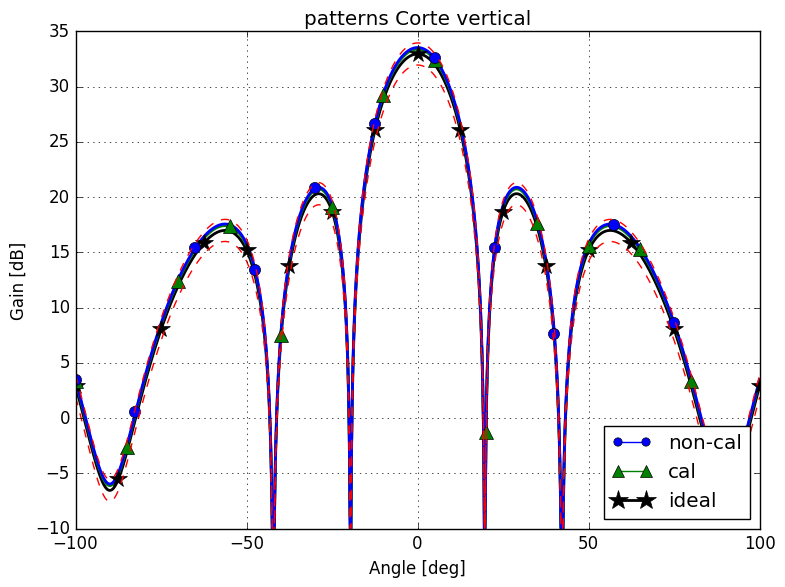
\includegraphics[width=7cm]{gfx/nonErrClassical10degColElCut.png}}
	\caption{Señales transmitidas por la antena en los casos deseado (ideal), pre (non-cal) y post (cal) calibración clásica.}
	\label{fig:nonErrClassical10degCol}
\end{figure}

La tabla \ref{tab:nonErrClassical10degCol} muestra como la ganancia relativa de los lóbulos secundarios con respecto al del lóbulo
principal de cada diagrama se mantienen invariantes e iguales al del diagrama ideal, 12.97 dBc en polarización H y 12.65 dBc en
polarización V. A su vez se puede observar que, dado que el esquema de calibración no abarca la totalidad del sistema, la
diferencia de la ganancia del diagrama calibrado disminuye pero no llega a ser igual a cero.

\begin{table}[H]
  \footnotesize
  \centering
  \begin{tabular}{|c|c|C{2cm}|C{2.5cm}|C{2.5cm}|C{2.5cm}|}
    \hline
    Caso & Corte & Ganancia - lóbulo izq. [dBc] & Ganancia - lóbulo central [dB] &
    Ganancia - lóbulo der. [dBc] & Ancho - lóbulo central -3dB \tabularnewline\hline
    \multirow{2}{2cm}{Diag. rad. sin calibrar} & H & 12.97 & 43.48 & 12.97 & 12.4 \tabularnewline\cline{2-6}
     & V & 12.65 & 33.54 & 12.65 & 17.4 \tabularnewline\hline
    \multirow{2}{2cm}{Diag. rad. calibrado} & H & 12.97 & 43.34 & 12.97 & 12.4 \tabularnewline\cline{2-6}
     & V & 12.65 & 33.4 & 12.65 & 17.4 \tabularnewline\hline
    \multirow{2}{2cm}{Diag. rad. ideal} & H & 12.97 & 42.9 & 12.97 & 12.4 \tabularnewline\cline{2-6}
     & V & 12.65 & 32.96 & 12.65 & 17.4 \tabularnewline\hline
    \multirow{2}{2cm}{Dif. sin calibrar} & H & 0.0 & 0.58 & 0.0 & 0.0\tabularnewline\cline{2-6}
     & V & 0.0 & 0.58 & 0.0 & 0.0 \tabularnewline\hline
    \multirow{2}{2cm}{Dif. calibrado} & H & 0.0 & 0.44 & 0.0 & 0.0 \tabularnewline\cline{2-6}
     & V & 0.0 & 0.44 & 0.0 & 0.0 \tabularnewline\hline
  \end{tabular}
  \caption{Propiedades de los diagramas de radiación calibrados y sin calibrar comparados con el ideal.}
  \label{tab:nonErrClassical10degCol}
\end{table}


\subsubsection{Apuntamiento 10 grados en rango (vertical)}

Los gráficos de la figura \ref{fig:nonErrClassical10degRow} muestran que el calibrador, por no abarcar la totalidad del sistema, no 
puede determinar correctamente ni la ganancia ni fase de la antena. Aun asi, como dicho desvío es el mismo para todos los
elementos el diagrama de radiación resultante mantiene su forma y sus atributos no se modifican, salvo la ganancia total.

Se observa que la ganancia es la misma en todos los elementos de antena, pero que la fase presenta una distribución escalonada
porque se está apuntado verticalmente, por ende, todos los elementos pertenecientes a una misma fila poseen la misma fase y entre
filas se presenta un desfase lineal porque la separación es uniforme. Por ejemplo, los ER número 0, 1, 2, 3, 4, 5, 6, 7, 8 y 9
pertenecientes al primer panel poseen una fase ideal aproximada a los -50 grados.

El desfase entre paneles depende de la inclinación del frente de onda deseado, la frecuencia de la señal utilizada y de la
separación entre elementos radiantes.

De los diagramas de radiación se observa el máximo en los cero grados para el corte horizontal y en diez grados para el corte
vertical y que los lóbulos secundarios se encuentran aproximadamente a 13 dBc por debajo de dichos máximos.

Los tres estados de señales graficados son el deseado (caso ideal), el previo a calibrar (non-cal) y el resultante de la
calibración (cal).

\begin{figure}[H]
	\centering
 	\subfloat[Ganancia y fase transmitida por cada ER]{
		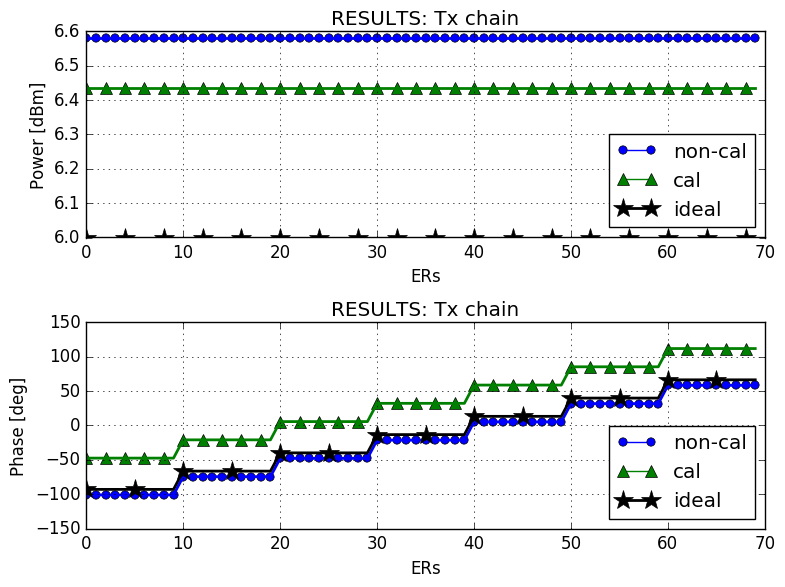
\includegraphics[width=9cm]{gfx/nonErrClassical10degRow.png}}

	\subfloat[Corte en azimut (horizontal) del diagrama de radiación]{
		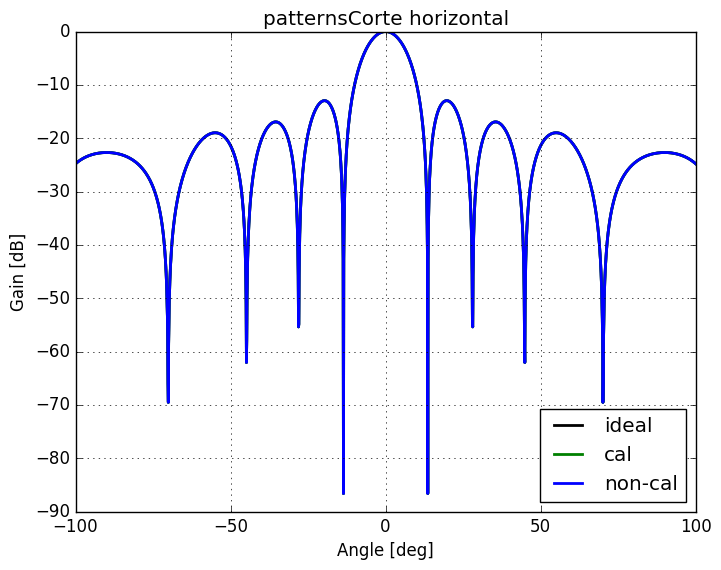
\includegraphics[width=7cm]{gfx/nonErrClassical10degRowAzCut.png}}
	\subfloat[Corte en rango (vertical) del diagrama de radiación]{
		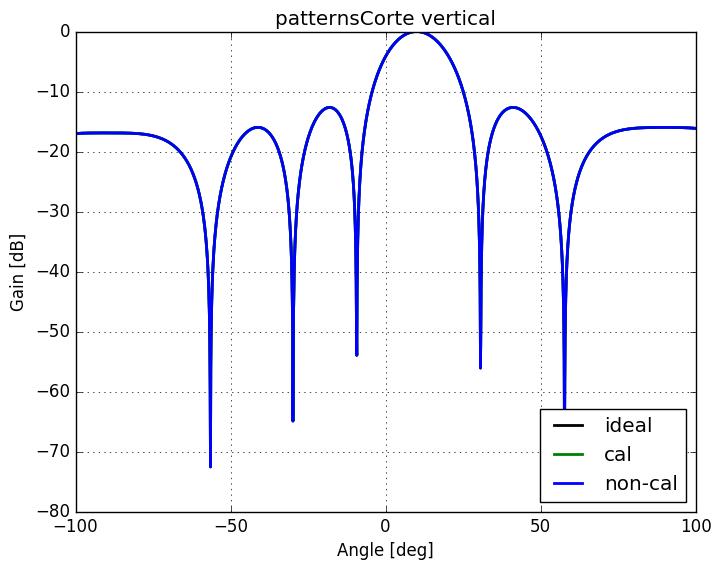
\includegraphics[width=7cm]{gfx/nonErrClassical10degRowElCut.png}}
	\caption{Señales transmitidas por la antena en los casos deseado (ideal), pre (non-cal) y post (cal) calibración clásica.}
	\label{fig:nonErrClassical10degRow}
\end{figure}
La tabla \ref{tab:nonErrClassical10degRow} muestra como la ganancia relativa de los lóbulos secundarios con respecto al del lóbulo
principal de cada diagrama se mantienen invariantes e iguales al del diagrama ideal, 12.97 dBc en polarización H y 12.65 dBc en
polarización V. A su vez se puede observar que, dado que el esquema de calibración no abarca la totalidad del sistema, la
diferencia de la ganancia del diagrama calibrado disminuye pero no llega a ser igual a cero.
\begin{table}[H]
  \footnotesize
  \centering
  \begin{tabular}{|c|c|C{2cm}|C{2.5cm}|C{2.5cm}|C{2.5cm}|}
    \hline
    Caso & Corte & Ganancia - lóbulo izq. [dBc] & Ganancia - lóbulo central [dB] &
    Ganancia - lóbulo der. [dBc] & Ancho - lóbulo central -3dB \tabularnewline\hline
    \multirow{2}{2cm}{Diag. rad. sin calibrar} & H & 12.97 & 39.34 & 12.97 & 12.0 \tabularnewline\cline{2-6}
     & V & 12.65 & 43.48 & 12.65 & 17.8 \tabularnewline\hline
    \multirow{2}{2cm}{Diag. rad. calibrado} & H & 12.97 & 39.19 & 12.97 & 12.0 \tabularnewline\cline{2-6}
     & V & 12.65 & 43.34 & 12.65 & 17.8 \tabularnewline\hline
    \multirow{2}{2cm}{Diag. rad. ideal} & H & 12.97 & 38.76 & 12.97 & 12.0 \tabularnewline\cline{2-6}
     & V & 12.65 & 42.9 & 12.65 & 17.8 \tabularnewline\hline
    \multirow{2}{2cm}{Dif. sin calibrar} & H & 0.0 & 0.58 & 0.0 & 0.0\tabularnewline\cline{2-6}
     & V & 0.0 & 0.58 & 0.0 & 0.0 \tabularnewline\hline
    \multirow{2}{2cm}{Dif. calibrado} & H & 0.0 & 0.43 & 0.0 & 0.0 \tabularnewline\cline{2-6}
     & V & 0.0 & 0.44 & 0.0 & 0.0 \tabularnewline\hline
  \end{tabular}
  \caption{Propiedades de los diagramas de radiación calibrados y sin calibrar comparados con el ideal.}
  \label{tab:nonErrClassical10degRow}
\end{table}


\subsection{Calibración por acoplamientos mutuos en el caso ideal}

A continuación se presentan los tres casos de prueba definidos en la sección \ref{sc:characteristics} para el método de
calibración por acoplamientos mutuos.


\subsubsection{Apuntamiento uniforme}

Los gráficos de la figura \ref{fig:nonErrMutual0deg} muestran que el calibrador funciona correctamente para estimar y corregir la 
fase y ganancia del sistema. Se observa que la ganancia y fase es la misma en todos los elementos radiantes de la antena e
iguales a los valores deseados.

De los diagramas de radiación se ve el máximo en el centro (cero grados de inclinación de apuntamiento) y se observan los
lóbulos secundarios a 12.97 dBc por debajo del lóbulo primario.

Los tres estados de señales graficados son el deseado (caso ideal), el previo a calibrar (non-cal) y el resultante de la
calibración (cal).

\begin{figure}[H]
	\centering
 	\subfloat[Ganancia y fase transmitida por cada ER]{
		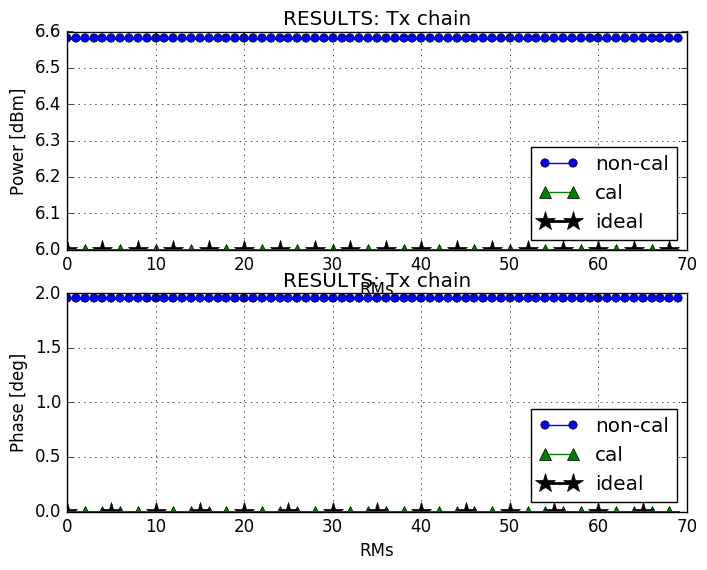
\includegraphics[width=9cm]{gfx/nonErrMutual0deg.png}}

	\subfloat[Corte en azimut (horizontal) del diagrama de radiación]{
		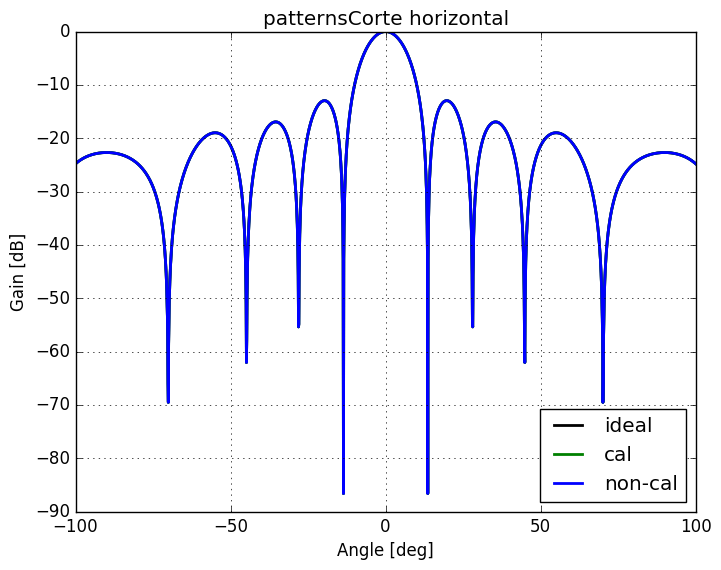
\includegraphics[width=7cm]{gfx/nonErrMutual0degAzCut.png}}
	\subfloat[Corte en rango (vertical) del diagrama de radiación]{
		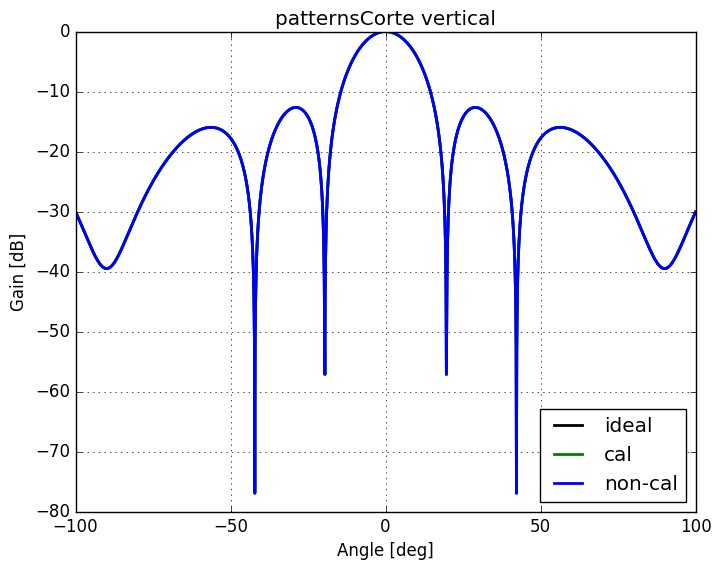
\includegraphics[width=7cm]{gfx/nonErrMutual0degElCut.png}}
	\caption{Señales transmitidas por la antena en los casos deseado (ideal), pre (non-cal) y post (cal) calibración por acoplamientos mutuos.}
	\label{fig:nonErrMutual0deg}
\end{figure}

La tabla \ref{tab:nonErrMutual0deg} muestra cómo la ganancia relativa de los lóbulos secundarios con respecto al del lóbulo
principal de cada diagrama se mantienen invariantes e iguales a los del diagrama ideal, 12.97 dBc en polarización H y 12.65 dBc
en polarización V. A su vez, se puede observar que la potencia del haz principal fue correctamente calibrada, resultando en 32.1
dBc para la polarización H y 53.96 dBc para la polarización vertical.

\begin{table}[H]
  \footnotesize
  \centering
  \begin{tabular}{|c|c|C{2cm}|C{2.5cm}|C{2.5cm}|C{2.5cm}|}
    \hline
    Caso & Corte & Ganancia - lóbulo izq. [dBc] & Ganancia - lóbulo central [dB] &
    Ganancia - lóbulo der. [dBc] & Ancho - lóbulo central -3dB \tabularnewline\hline
    \multirow{2}{2cm}{Diag. rad. sin calibrar} & H & 12.97 & 43.48 & 12.97 & 12.0 \tabularnewline\cline{2-6}
     & V & 12.65 & 43.48 & 12.65 & 17.4 \tabularnewline\hline
    \multirow{2}{2cm}{Diag. rad. calibrado} & H & 12.97 & 42.9 & 12.97 & 12.0 \tabularnewline\cline{2-6}
     & V & 12.65 & 42.9 & 12.65 & 17.4 \tabularnewline\hline
    \multirow{2}{2cm}{Diag. rad. ideal} & H & 12.97 & 42.9 & 12.97 & 12.0 \tabularnewline\cline{2-6}
     & V & 12.65 & 42.9 & 12.65 & 17.4 \tabularnewline\hline
    \multirow{2}{2cm}{Dif. sin calibrar} & H & 0.0 & 0.58 & 0.0 & 0.0\tabularnewline\cline{2-6}
     & V & 0.0 & 0.58 & 0.0 & 0.0 \tabularnewline\hline
    \multirow{2}{2cm}{Dif. calibrado} & H & 0.0 & 0.0 & 0.0 & 0.0 \tabularnewline\cline{2-6}
     & V & 0.0 & 0.0 & 0.0 & 0.0 \tabularnewline\hline
  \end{tabular}
  \caption{Propiedades de los diagramas de radiación calibrados y sin calibrar comparados con el ideal.}
  \label{tab:nonErrMutual0deg}
\end{table}


\subsubsection{Apuntamiento 10 grados en azimut (horizontal)}

Los gráficos de la figura \ref{fig:nonErrMutual10degCol} muestran que el calibrador funciona correctamente para estimar y 
corregir la fase y ganancia del sistema utilizando un apuntamiento diferente al uniforme logrando así que los diagramas de 
radiación calibrados resultan iguales al ideal. 

Se observa que la ganancia es la misma en todos los elementos de antena, pero que la fase presenta una distribución diente de
sierra porque se está apuntado horizontalmente, por ende, todos los elementos que pertenecen a un mismo panel, o columna, poseen
la misma fase y entre paneles hay un desfase lineal porque la separación es uniforme. Por ejemplo, los ER número 3, 13, 23, 33,
43, 53 y 63, pertenecientes al segundo panel, poseen una fase ideal aproximada a los -60 grados.

El desfase entre paneles depende de la inclinación del frente de onda deseado, la frecuencia de la señal utilizada y de la
separación entre elementos radiantes.

De los diagramas de radiación se observa el máximo en los diez grados para el corte horizontal y en cero grados para el corte
vertical y que los lóbulos secundarios se encuentran aproximadamente a 13 dBc por debajo de dichos máximos.

Los tres estados de señales graficados son el deseado (caso ideal), el previo a calibrar (non-cal) y el resultante de la
calibración (cal).
\begin{figure}[H]
	\centering
 	\subfloat[Ganancia y fase transmitida por cada ER]{
		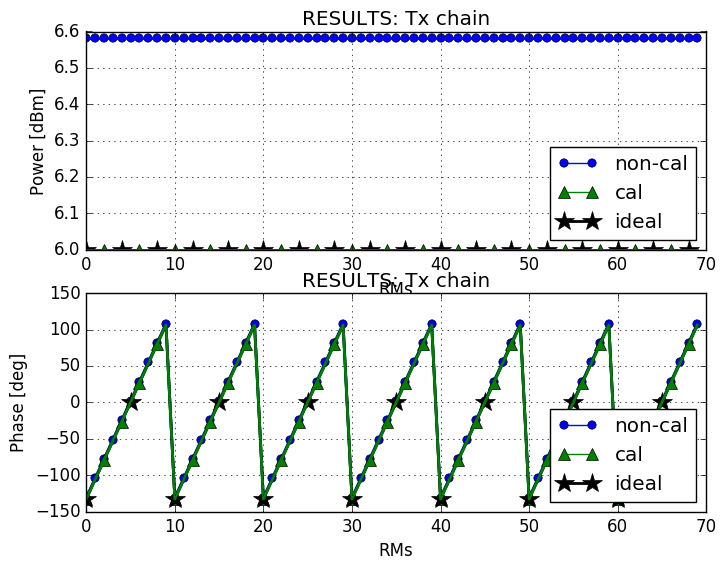
\includegraphics[width=9cm]{gfx/nonErrMutual10degCol.png}}

	\subfloat[Corte en azimut (horizontal) del diagrama de radiación]{
		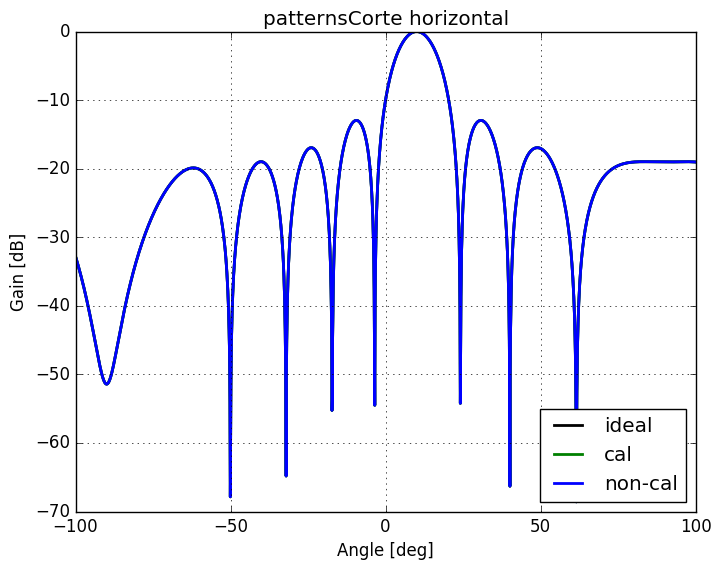
\includegraphics[width=7cm]{gfx/nonErrMutual10degColAzCut.png}}
	\subfloat[Corte en rango (vertical) del diagrama de radiación]{
		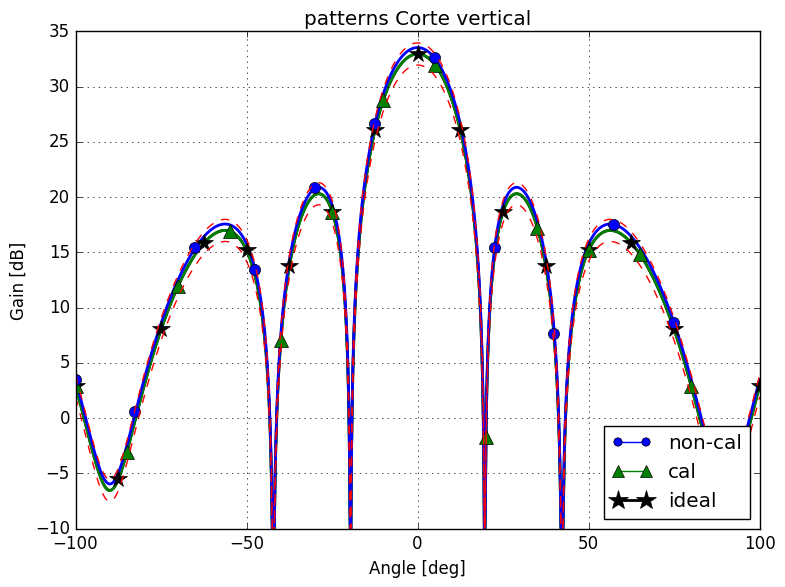
\includegraphics[width=7cm]{gfx/nonErrMutual10degColElCut.png}}
	\caption{Señales transmitidas por la antena en los casos deseado (ideal), pre (non-cal) y post (cal) calibración por acoplamientos mutuos.}
	\label{fig:nonErrMutual10degCol}
\end{figure}
La tabla \ref{tab:nonErrMutual10degCol} muestra cómo la ganancia relativa de los lóbulos secundarios con respecto al del lóbulo
principal de cada diagrama se mantienen invariantes e iguales a los del diagrama ideal, 12.97 dBc en polarización H y 12.65 dBc
en polarización V. A su vez, se puede observar que la potencia del haz principal fue correctamente calibrada, resultando en 42.9
dBc para la polarización H y 32.96 dBc para la polarización vertical.
\begin{table}[H]
  \footnotesize
  \centering
  \begin{tabular}{|c|c|C{2cm}|C{2.5cm}|C{2.5cm}|C{2.5cm}|}
    \hline
    Caso & Corte & Ganancia - lóbulo izq. [dBc] & Ganancia - lóbulo central [dB] &
    Ganancia - lóbulo der. [dBc] & Ancho - lóbulo central -3dB \tabularnewline\hline
    \multirow{2}{2cm}{Diag. rad. sin calibrar} & H & 12.97 & 43.48 & 12.97 & 12.4 \tabularnewline\cline{2-6}
     & V & 12.65 & 33.54 & 12.65 & 17.4 \tabularnewline\hline
    \multirow{2}{2cm}{Diag. rad. calibrado} & H & 12.97 & 42.9 & 12.97 & 12.4 \tabularnewline\cline{2-6}
     & V & 12.65 & 32.96 & 12.65 & 17.4 \tabularnewline\hline
    \multirow{2}{2cm}{Diag. rad. ideal} & H & 12.97 & 42.9 & 12.97 & 12.4 \tabularnewline\cline{2-6}
     & V & 12.65 & 32.96 & 12.65 & 17.4 \tabularnewline\hline
    \multirow{2}{2cm}{Dif. sin calibrar} & H & 0.0 & 0.58 & 0.0 & 0.0\tabularnewline\cline{2-6}
     & V & 0.0 & 0.58 & 0.0 & 0.0 \tabularnewline\hline
    \multirow{2}{2cm}{Dif. calibrado} & H & 0.0 & 0.0 & 0.0 & 0.0 \tabularnewline\cline{2-6}
     & V & 0.0 & 0.0 & 0.0 & 0.0 \tabularnewline\hline
  \end{tabular}
  \caption{Propiedades de los diagramas de radiación calibrados y sin calibrar comparados con el ideal.}
  \label{tab:nonErrMutual10degCol}
\end{table}


\subsubsection{Apuntamiento 10 grados en rango (vertical)}

Los gráficos de la figura \ref{fig:nonErrMutual10degRow} muestran que el calibrador funciona correctamente para estimar y 
corregir la fase y ganancia del sistema utilizando un apuntamiento diferente al uniforme logrando así que los diagramas de 
radiación calibrados resultan iguales al ideal.

Los gráficos de la figura \ref{fig:nonErrClassical10degRow} muestran que el calibrador, por no abarcar la totalidad del sistema, no 
puede determinar correctamente ni la ganancia ni fase de la antena. Aun así, como dicho desvío es el mismo para todos los
elementos el diagrama de radiación resultante mantiene su forma y sus atributos no se modifican, salvo la ganancia total.

Se observa que la ganancia es la misma en todos los elementos de antena, pero que la fase presenta una distribución escalonada
porque se está apuntado verticalmente, por ende, todos los elementos pertenecientes a una misma fila poseen la misma fase y entre
filas se presenta un desfase lineal porque la separación es uniforme. Por ejemplo, los ER número 0, 1, 2, 3, 4, 5, 6, 7, 8 y 9
pertenecientes al primer panel poseen una fase ideal aproximada a los -100 grados.

El desfase entre paneles depende de la inclinación del frente de onda deseado, la frecuencia de la señal utilizada y de la
separación entre elementos radiantes.

De los diagramas de radiación se observa el máximo en los cero grados para el corte horizontal y en diez grados para el corte
vertical y que los lóbulos secundarios se encuentran aproximadamente a 13 dBc por debajo de dichos máximos.

Los tres estados de señales graficados son el deseado (caso ideal), el previo a calibrar (non-cal) y el resultante de la
calibración (cal).

\begin{figure}[H]
	\centering
 	\subfloat[Ganancia y fase transmitida por cada ER]{
		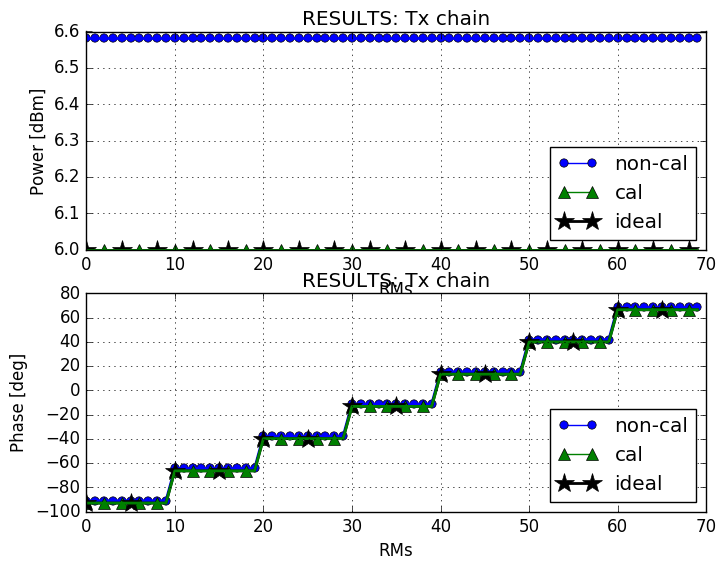
\includegraphics[width=9cm]{gfx/nonErrMutual10degRow.png}}

	\subfloat[Corte en azimut (horizontal) del diagrama de radiación]{
		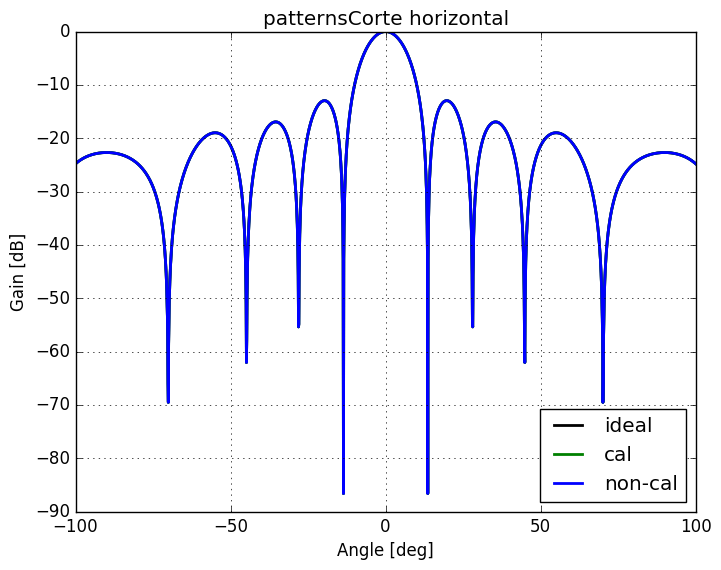
\includegraphics[width=7cm]{gfx/nonErrMutual10degRowAzCut.png}}
	\subfloat[Corte en rango (vertical) del diagrama de radiación]{
		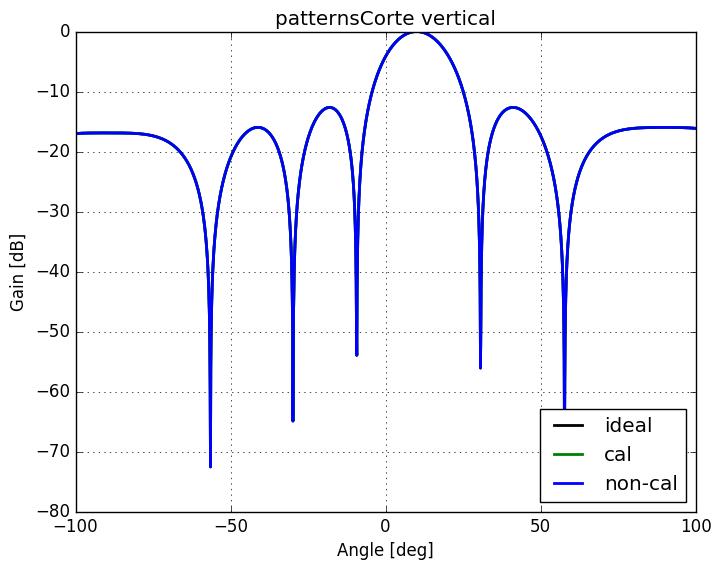
\includegraphics[width=7cm]{gfx/nonErrMutual10degRowElCut.png}}
	\caption{Señales transmitidas por la antena en los casos deseado (ideal), pre (non-cal) y post (cal) calibración por acoplamientos mutuos.}
	\label{fig:nonErrMutual10degRow}
\end{figure}
La tabla \ref{tab:nonErrMutual10degRow} muestra cómo la ganancia relativa de los lóbulos secundarios con respecto al del lóbulo
principal de cada diagrama se mantienen invariantes e iguales a los del diagrama ideal, 12.97 dBc en polarización H y 12.65 dBc
en polarización V. A su vez, se puede observar que la potencia del haz principal fue correctamente calibrada, resultando en 38.76
dBc para la polarización H y 42.9 dBc para la polarización vertical.
\begin{table}[H]
  \footnotesize
  \centering
  \begin{tabular}{|c|c|C{2cm}|C{2.5cm}|C{2.5cm}|C{2.5cm}|}
    \hline
    Caso & Corte & Ganancia - lóbulo izq. [dBc] & Ganancia - lóbulo central [dB] &
    Ganancia - lóbulo der. [dBc] & Ancho - lóbulo central -3dB \tabularnewline\hline
    \multirow{2}{2cm}{Diag. rad. sin calibrar} & H & 12.97 & 39.34 & 12.97 & 12.0 \tabularnewline\cline{2-6}
     & V & 12.65 & 43.48 & 12.65 & 17.8 \tabularnewline\hline
    \multirow{2}{2cm}{Diag. rad. calibrado} & H & 12.97 & 38.76 & 12.97 & 12.0 \tabularnewline\cline{2-6}
     & V & 12.65 & 42.9 & 12.65 & 17.8 \tabularnewline\hline
    \multirow{2}{2cm}{Diag. rad. ideal} & H & 12.97 & 38.76 & 12.97 & 12.0 \tabularnewline\cline{2-6}
     & V & 12.65 & 42.9 & 12.65 & 17.8 \tabularnewline\hline
    \multirow{2}{2cm}{Dif. sin calibrar} & H & 0.0 & 0.58 & 0.0 & 0.0\tabularnewline\cline{2-6}
     & V & 0.0 & 0.58 & 0.0 & 0.0 \tabularnewline\hline
    \multirow{2}{2cm}{Dif. calibrado} & H & 0.0 & 0.0 & 0.0 & 0.0 \tabularnewline\cline{2-6}
     & V & 0.0 & 0.0 & 0.0 & 0.0 \tabularnewline\hline
  \end{tabular}
  \caption{Propiedades de los diagramas de radiación calibrados y sin calibrar comparados con el ideal.}
  \label{tab:nonErrMutual10degRow}
\end{table}


\section{TRMs dañados}
\label{sc:trmsDamaged} 

Los casos de simulación de esta sección tienen las siguientes caracterísiticas,
\begin{itemize}
	\item Salvo tres TRMs que están dañados, el resto de los componentes de antena no tienen ningún problema de funcionamiento ni 
		desadaptaciones. Las posiciones de los TRMs son: [1,0], [3,4] y [5,5]. La nomenclatura de lectura es [fila, columna] con 
		valores desde 0.
	\item No hay dispersiones en el comportamiento del resto de componentes.
	\item No hay dispersiones en la señal, la misma es invariante en el tiempo.
\end{itemize}

\subsection{Calibración clásica con TRMs dañados}

A continuación se presentan los tres casos de prueba definidos en la sección \ref{sc:characteristics} para el método de
calibración interna clásico.


\subsubsection{Apuntamiento uniforme}

Los gráficos de la figura \ref{fig:deadTRMsClassical0deg} muestran que el calibrador, dejando de lado la diferencia de 
estimación tanto de fase como ganancia por no abarcar la totalidad del sistema, funciona correctamente. Los elementos 10, 34 y 
55 presentan una ganancia que equivaldría al piso de ruido.

Analizando los diagramas de radiación, se observa que debido a la causa de TRMs dañados, se aprecia un aumento considerable de
ambos lóbulos secundarios del corte horizontal, generando así que la diferencia con el lóbulo principal sea menor. El corte
vertical no presenta grandes desvíos.

Los tres estados de señales graficados son el deseado (caso ideal), el previo a calibrar (non-cal) y el resultante de la
calibración (cal).
\begin{figure}[H]
	\centering
 	\subfloat[Ganancia y fase transmitida por cada ER]{
		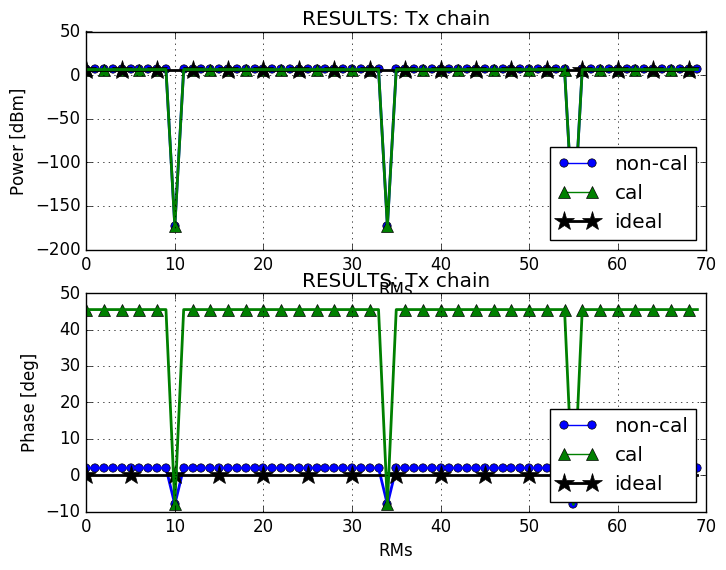
\includegraphics[width=9cm]{gfx/deadTRMsClassical0deg.png}}

	\subfloat[Corte en azimut (horizontal) del diagrama de radiación]{
		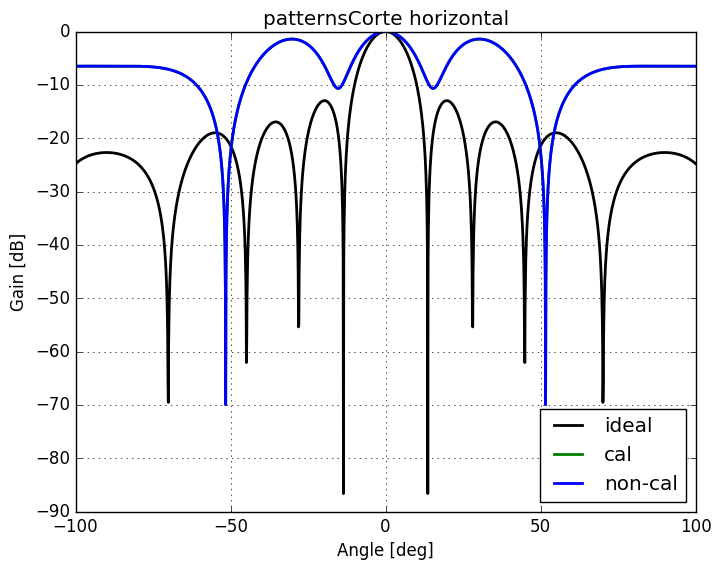
\includegraphics[width=7cm]{gfx/deadTRMsClassical0degAzCut.png}}
	\subfloat[Corte en rango (vertical) del diagrama de radiación]{
		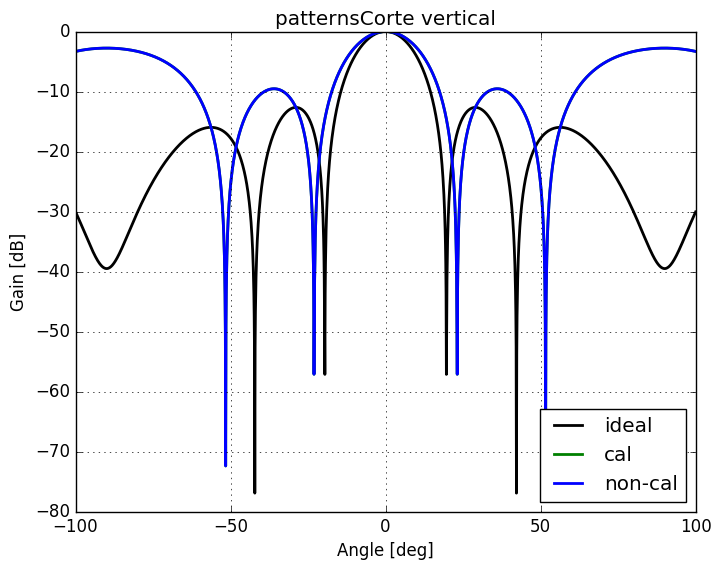
\includegraphics[width=7cm]{gfx/deadTRMsClassical0degElCut.png}}
	\caption{Señales transmitidas por la antena en los casos deseado (ideal), pre (non-cal) y post (cal) calibración clásica.}
	\label{fig:deadTRMsClassical0deg}
\end{figure}

La tabla \ref{tab:deadTRMsClassical0deg} muestra que las diferencias de ganancia de los lóbulos secundarios entre los diagramas 
reales y el ideal para el corte horizontal es de -0.66 dB, el signo negativo indica que el lóbulo del diagrama calibrado es mayor
que el ideal. En el corte vertical dicha diferencia es casi la mitad, de 0.38 dB. A su vez, se puede apreciar que la diferencia
en la ganancia del lóbulo principal se disminuyó a los 0.06 dB.

\begin{table}[H]
  \footnotesize
  \centering
  \begin{tabular}{|c|c|C{2cm}|C{2.5cm}|C{2.5cm}|C{2.5cm}|}
    \hline
    Caso & Corte & Ganancia - lóbulo izq. [dBc] & Ganancia - lóbulo central [dB] &
    Ganancia - lóbulo der. [dBc] & Ancho - lóbulo central -3dB \tabularnewline\hline
    \multirow{2}{2cm}{Diag. rad. sin calibrar} & H & 12.31 & 43.1 & 12.31 & 12.0 \tabularnewline\cline{2-6}
     & V & 13.03 & 43.1 & 13.03 & 17.2 \tabularnewline\hline
    \multirow{2}{2cm}{Diag. rad. calibrado} & H & 12.31 & 42.96 & 12.31 & 12.0 \tabularnewline\cline{2-6}
     & V & 13.03 & 42.96 & 13.03 & 17.2 \tabularnewline\hline
    \multirow{2}{2cm}{Diag. rad. ideal} & H & 12.97 & 42.9 & 12.97 & 12.0 \tabularnewline\cline{2-6}
     & V & 12.65 & 42.9 & 12.65 & 17.4 \tabularnewline\hline
    \multirow{2}{2cm}{Dif. sin calibrar} & H & -0.66 & 0.2 & -0.66 & 0.0\tabularnewline\cline{2-6}
     & V & 0.38 & 0.2 & 0.38 & -0.2 \tabularnewline\hline
    \multirow{2}{2cm}{Dif. calibrado} & H & -0.66 & 0.06 & -0.66 & 0.0 \tabularnewline\cline{2-6}
     & V & 0.38 & 0.06 & 0.38 & -0.2 \tabularnewline\hline
  \end{tabular}
  \caption{Propiedades de los diagramas de radiación calibrados y sin calibrar comparados con el ideal.}
  \label{tab:deadTRMsClassical0deg}
\end{table}


\subsubsection{Apuntamiento 10 grados en azimut (horizontal)}

Los gráficos de la figura \ref{fig:deadTRMsClassical10degCol} muestran que el calibrador, dejando de lado la diferencia de 
estimación tanto de fase como ganancia por no abarcar la totalidad del sistema, funciona correctamente. Los elementos 10, 34 y 
55 presentan una ganancia que equivaldría al piso de ruido.

Analizando los diagramas de radiación, se observa que debido a la causa de TRMs dañados, se aprecia un aumento considerable de
ambos lóbulos secundarios del corte horizontal, generando así que la diferencia con el lóbulo principal sea menor. En el corte
vertical se aprecia que el segundo lóbulo secundario derecho del diagrama calibrado supera por más de un dB en ganancia al
primero, este incremento en ganancia resulta inadmisible.

Los tres estados de señales graficados son el deseado (caso ideal), el previo a calibrar (non-cal) y el resultante de la
calibración (cal).
\begin{figure}[H]
	\centering
 	\subfloat[Ganancia y fase transmitida por cada ER]{
		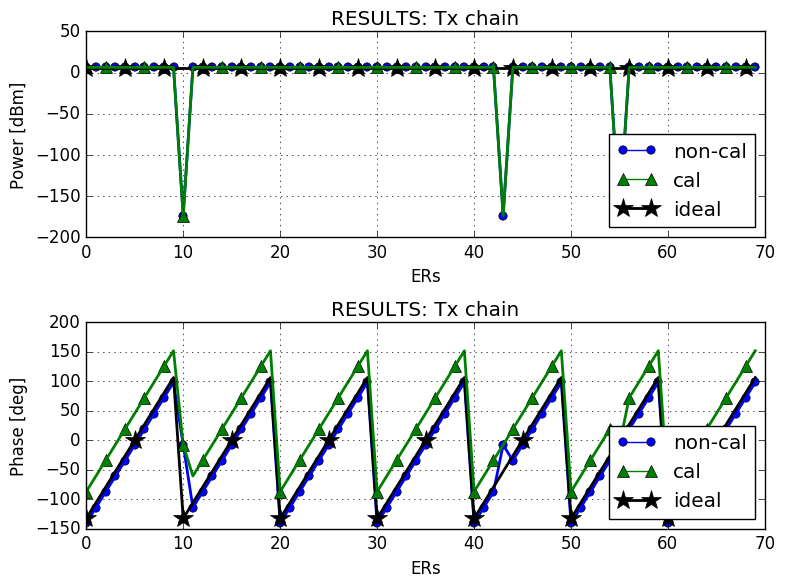
\includegraphics[width=9cm]{gfx/deadTRMsClassical10degCol.png}}

	\subfloat[Corte en azimut (horizontal) del diagrama de radiación]{
		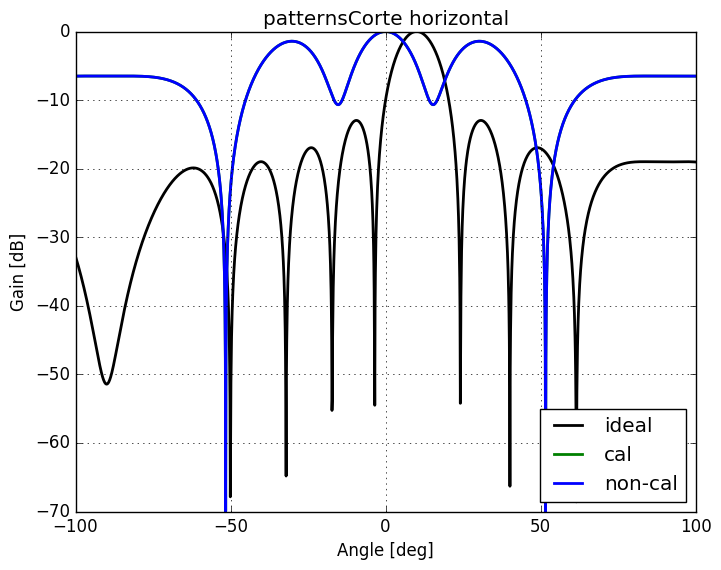
\includegraphics[width=7cm]{gfx/deadTRMsClassical10degColAzCut.png}}
	\subfloat[Corte en rango (vertical) del diagrama de radiación]{
		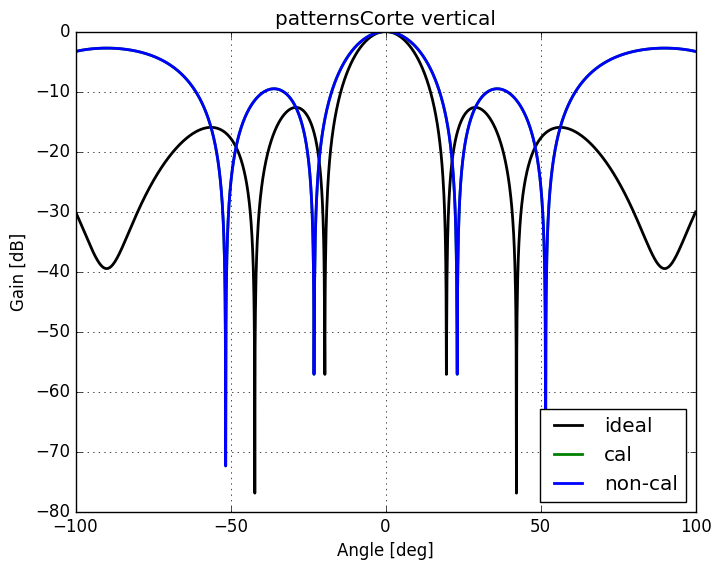
\includegraphics[width=7cm]{gfx/deadTRMsClassical10degColElCut.png}}
	\caption{Señales transmitidas por la antena en los casos deseado (ideal), pre (non-cal) y post (cal) calibración clásica.}
	\label{fig:deadTRMsClassical10degCol}
\end{figure}
La tabla \ref{tab:deadTRMsClassical10degCol} muestra que las diferencias de ganancia de los lóbulos secundarios entre los 
diagramas de radiación reales y el ideal para el corte horizontal es de -0.66 dB, el signo negativo indica que el lóbulo del
diagrama calibrado es mayor que el ideal. En el corte vertical dicha diferencia es de -0.78 dB. A su vez, se puede apreciar que
la diferencia en la ganancia del lóbulo principal en ambos cortes se disminuyó a los 0.06 dB y -0.04 dB respectivamente. Por
último, el ancho del lóbulo principal se ve levemente ensanchado, resultando en 0.2 grados más ancho que el ideal.
\begin{table}[H]
  \footnotesize
  \centering
  \begin{tabular}{|c|c|C{2cm}|C{2.5cm}|C{2.5cm}|C{2.5cm}|}
    \hline
    Caso & Corte & Ganancia - lóbulo izq. [dBc] & Ganancia - lóbulo central [dB] &
    Ganancia - lóbulo der. [dBc] & Ancho - lóbulo central -3dB \tabularnewline\hline
    \multirow{2}{2cm}{Diag. rad. sin calibrar} & H & 12.31 & 43.1 & 12.31 & 12.4 \tabularnewline\cline{2-6}
     & V & 11.87 & 33.06 & 12.13 & 17.2 \tabularnewline\hline
    \multirow{2}{2cm}{Diag. rad. calibrado} & H & 12.31 & 42.96 & 12.31 & 12.4 \tabularnewline\cline{2-6}
     & V & 11.87 & 32.92 & 12.13 & 17.2 \tabularnewline\hline
    \multirow{2}{2cm}{Diag. rad. ideal} & H & 12.97 & 42.9 & 12.97 & 12.4 \tabularnewline\cline{2-6}
     & V & 12.65 & 32.96 & 12.65 & 17.4 \tabularnewline\hline
    \multirow{2}{2cm}{Dif. sin calibrar} & H & -0.66 & 0.2 & -0.66 & 0.0\tabularnewline\cline{2-6}
     & V & -0.78 & 0.1 & -0.52 & -0.2 \tabularnewline\hline
    \multirow{2}{2cm}{Dif. calibrado} & H & -0.66 & 0.06 & -0.66 & 0.0 \tabularnewline\cline{2-6}
     & V & -0.78 & -0.04 & -0.52 & -0.2 \tabularnewline\hline
  \end{tabular}
  \caption{Propiedades de los diagramas de radiación calibrados y sin calibrar comparados con el ideal.}
  \label{tab:deadTRMsClassical10degCol}
\end{table}


\subsubsection{Apuntamiento 10 grados en rango (vertical)}

Los gráficos de la figura \ref{fig:deadTRMsClassical10degRow} muestran que el calibrador, dejando de lado la diferencia de 
estimación tanto de fase como ganancia por no abarcar la totalidad del sistema, funciona correctamente. Los elementos 10, 34 y 
55 presentan una ganancia que equivaldría al piso de ruido.

Analizando los diagramas de radiación, se observa que debido a la causa de TRMs dañados, se aprecia un aumento considerable de
ambos lóbulos secundarios del corte horizontal, generando así que la diferencia con el lóbulo principal sea menor. En el corte
vertical no se aprecia tal diferencia. 

Los tres estados de señales graficados son el deseado (caso ideal), el previo a calibrar (non-cal) y el resultante de la
calibración (cal). 
\begin{figure}[H]
	\centering
 	\subfloat[Ganancia y fase transmitida por cada ER]{
		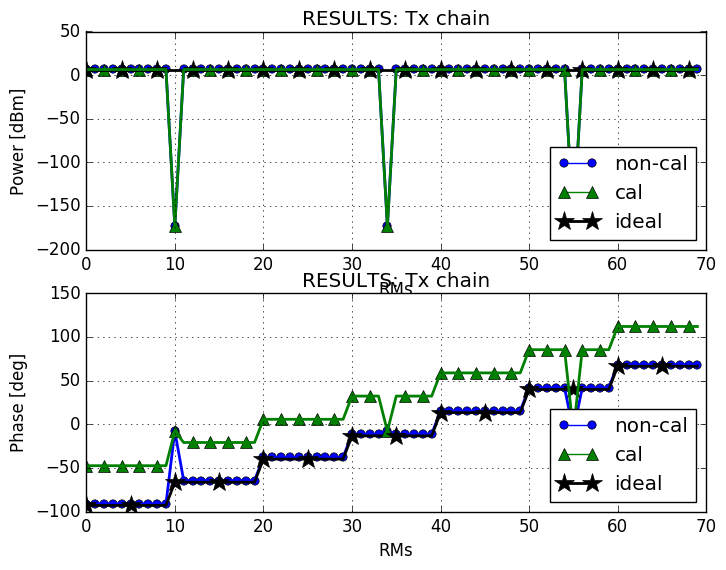
\includegraphics[width=9cm]{gfx/deadTRMsClassical10degRow.png}}

	\subfloat[Corte en azimut (horizontal) del diagrama de radiación]{
		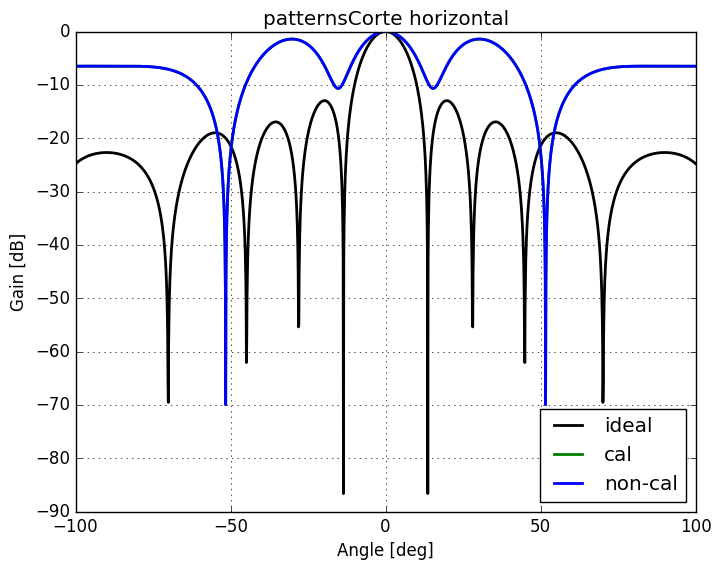
\includegraphics[width=7cm]{gfx/deadTRMsClassical10degRowAzCut.png}}
	\subfloat[Corte en rango (vertical) del diagrama de radiación]{
		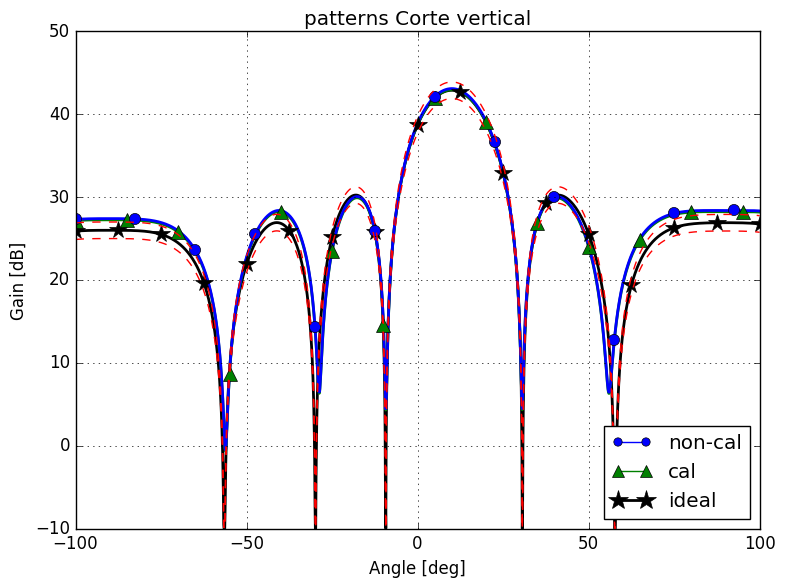
\includegraphics[width=7cm]{gfx/deadTRMsClassical10degRowElCut.png}}
	\caption{Señales transmitidas por la antena en los casos deseado (ideal), pre (non-cal) y post (cal) calibración clásica.}
	\label{fig:deadTRMsClassical10degRow}
\end{figure}

La tabla \ref{tab:deadTRMsClassical10degRow} muestra que las diferencias de ganancia de los lóbulos secundarios entre los 
diagramas de radiación reales y el ideal para el corte horizontal es de -1.41 dB (dicho valor es mayor que el admisible, 1 dB),
el signo negativo indica que la ganancia del lóbulo del diagrama calibrado es mayor que el ideal. En el corte vertical dicha
diferencia es de 0.38 dB. A su vez, se puede apreciar que la ganancia del lóbulo principal en el corte horizontal es igual al
ideal y el del corte vertical es 0.06 dB mayor. Por último, el ancho de los lóbulos principales no se ven afectados.

\begin{table}[H]
  \footnotesize
  \centering
  \begin{tabular}{|c|c|C{2cm}|C{2.5cm}|C{2.5cm}|C{2.5cm}|}
    \hline
    Caso & Corte & Ganancia - lóbulo izq. [dBc] & Ganancia - lóbulo central [dB] &
    Ganancia - lóbulo der. [dBc] & Ancho - lóbulo central -3dB \tabularnewline\hline
    \multirow{2}{2cm}{Diag. rad. sin calibrar} & H & 11.56 & 38.91 & 12.75 & 12.0 \tabularnewline\cline{2-6}
     & V & 13.03 & 43.1 & 13.03 & 17.8 \tabularnewline\hline
    \multirow{2}{2cm}{Diag. rad. calibrado} & H & 11.56 & 38.76 & 12.75 & 12.0 \tabularnewline\cline{2-6}
     & V & 13.03 & 42.96 & 13.03 & 17.8 \tabularnewline\hline
    \multirow{2}{2cm}{Diag. rad. ideal} & H & 12.97 & 38.76 & 12.97 & 12.0 \tabularnewline\cline{2-6}
     & V & 12.65 & 42.9 & 12.65 & 17.8 \tabularnewline\hline
    \multirow{2}{2cm}{Dif. sin calibrar} & H & -1.41 & 0.15 & -0.22 & 0.0\tabularnewline\cline{2-6}
     & V & 0.38 & 0.2 & 0.38 & 0.0 \tabularnewline\hline
    \multirow{2}{2cm}{Dif. calibrado} & H & -1.41 & 0.0 & -0.22 & 0.0 \tabularnewline\cline{2-6}
     & V & 0.38 & 0.06 & 0.38 & 0.0 \tabularnewline\hline
  \end{tabular}
  \caption{Propiedades de los diagramas de radiación calibrados y sin calibrar comparados con el ideal.}
  \label{tab:deadTRMsClassical10degRow}
\end{table}


\subsection{Calibración por acoplamientos mutuos con TRMs dañados}

A continuación se presentan los tres casos de prueba definidos en la sección \ref{sc:characteristics} para el método de
calibración por acoplamientos mutuos.


\subsubsection{Apuntamiento uniforme}

Los gráficos de la figura \ref{fig:deadTRMsMutual0deg} muestran que el calibrador funciona correctamente. Los elementos 10, 
34 y 55 presentan una ganancia que equivaldría al piso de ruido.

Analizando los diagramas de radiación, se observa que debido a la causa de trms dañados, se aprecia un aumento de
ambos lóbulos secundarios del corte horizontal, generando así que la diferencia con el lóbulo principal sea menor. el corte
vertical no presenta grandes desvíos.

Los tres estados de señales graficados son el deseado (caso ideal), el previo a calibrar (non-cal) y el resultante de la
calibración (cal). 
\begin{figure}[H]
	\centering
 	\subfloat[Ganancia y fase transmitida por cada ER]{
		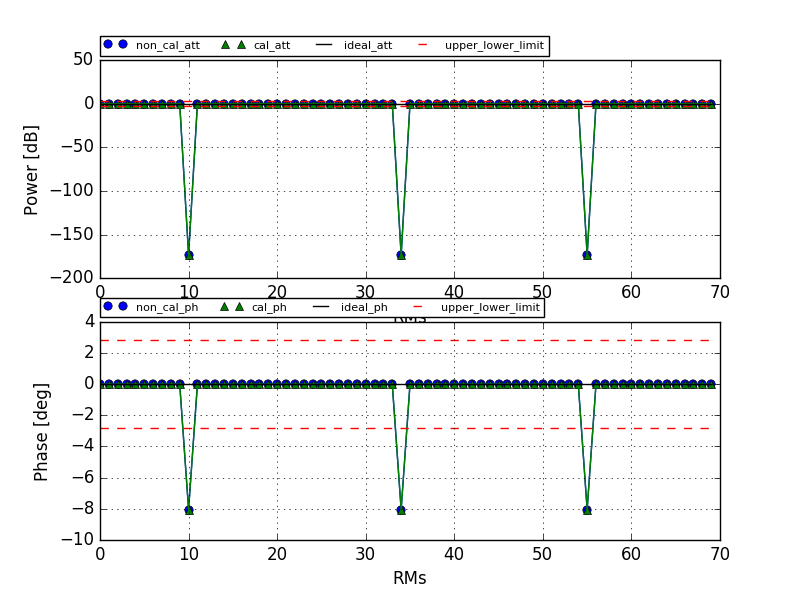
\includegraphics[width=9cm]{gfx/deadTRMsMutual0deg.png}}

	\subfloat[Corte en azimut (horizontal) del diagrama de radiación]{
		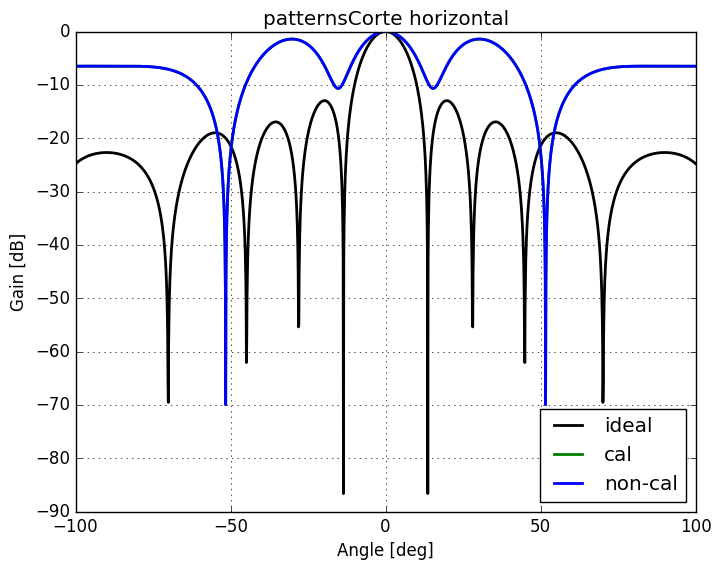
\includegraphics[width=7cm]{gfx/deadTRMsMutual0degAzCut.png}}
	\subfloat[Corte en rango (vertical) del diagrama de radiación]{
		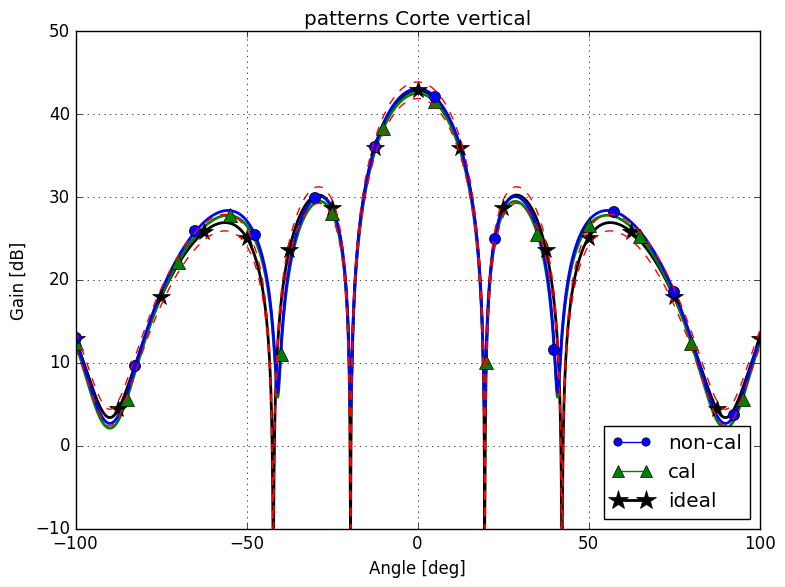
\includegraphics[width=7cm]{gfx/deadTRMsMutual0degElCut.png}}
	\caption{Señales transmitidas por la antena en los casos deseado (ideal), pre (non-cal) y post (cal) calibración por acoplamientos mutuos.}
	\label{fig:deadTRMsMutual0deg}
\end{figure}
La tabla \ref{tab:deadTRMsMutual0deg} muestra que las diferencias de ganancia de los lóbulos secundarios entre los diagramas 
reales y el ideal para el corte horizontal es de -0.66 dB, el signo negativo indica que el lóbulo del diagrama calibrado es mayor
que el ideal. En el corte vertical dicha diferencia es casi la mitad, de 0.38 dB. A su vez, se puede apreciar que la diferencia
en la ganancia del lóbulo principal se disminuyó a los -0.38 dB y que el ancho del mismo en el corte vertical es 0.2 grados mayor.
\begin{table}[H]
  \footnotesize
  \centering
  \begin{tabular}{|c|c|C{2cm}|C{2.5cm}|C{2.5cm}|C{2.5cm}|}
    \hline
    Caso & Corte & Ganancia - lóbulo izq. [dBc] & Ganancia - lóbulo central [dB] &
    Ganancia - lóbulo der. [dBc] & Ancho - lóbulo central -3dB \tabularnewline\hline
    \multirow{2}{2cm}{Diag. rad. sin calibrar} & H & 12.31 & 43.1 & 12.31 & 12.0 \tabularnewline\cline{2-6}
     & V & 13.03 & 43.1 & 13.03 & 17.2 \tabularnewline\hline
    \multirow{2}{2cm}{Diag. rad. calibrado} & H & 12.31 & 42.52 & 12.31 & 12.0 \tabularnewline\cline{2-6}
     & V & 13.03 & 42.52 & 13.03 & 17.2 \tabularnewline\hline
    \multirow{2}{2cm}{Diag. rad. ideal} & H & 12.97 & 42.9 & 12.97 & 12.0 \tabularnewline\cline{2-6}
     & V & 12.65 & 42.9 & 12.65 & 17.4 \tabularnewline\hline
    \multirow{2}{2cm}{Dif. sin calibrar} & H & -0.66 & 0.2 & -0.66 & 0.0\tabularnewline\cline{2-6}
     & V & 0.38 & 0.2 & 0.38 & -0.2 \tabularnewline\hline
    \multirow{2}{2cm}{Dif. calibrado} & H & -0.66 & -0.38 & -0.66 & 0.0 \tabularnewline\cline{2-6}
     & V & 0.38 & -0.38 & 0.38 & -0.2 \tabularnewline\hline
  \end{tabular}
  \caption{Propiedades de los diagramas de radiación calibrados y sin calibrar comparados con el ideal.}
  \label{tab:deadTRMsMutual0deg}
\end{table}


\subsubsection{Apuntamiento 10 grados en azimut (horizontal)}

Los gráficos de la figura \ref{fig:deadTRMsMutual10degCol} muestran que el calibrador funciona correctamente. Los elementos 10, 
34 y 55 presentan una ganancia que equivaldría al piso de ruido.

Analizando los diagramas de radiación, se observa que debido a la causa de TRMs dañados, se aprecia un aumento considerable de
ambos lóbulos secundarios de los cortes horizontal y vertical, generando así que las diferencias con el lóbulo principal sean
menores. En el corte vertical se aprecia que el segundo lóbulo secundario derecho del diagrama calibrado supera por más de un
dB en ganancia al primero, este incremento en ganancia resulta inadmisible.

Los tres estados de señales graficados son el deseado (caso ideal), el previo a calibrar (non-cal) y el resultante de la
calibración (cal). 
\begin{figure}[H]
	\centering
 	\subfloat[Ganancia y fase transmitida por cada ER]{
		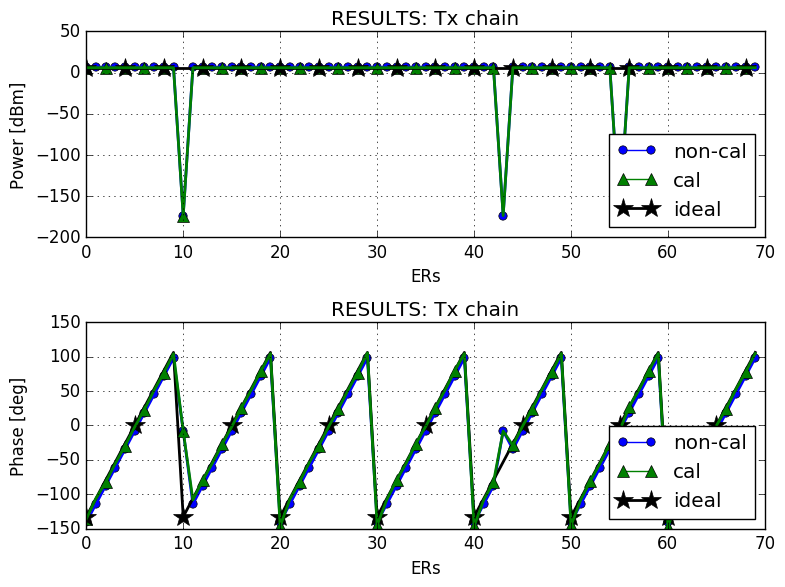
\includegraphics[width=9cm]{gfx/deadTRMsMutual10degCol.png}}

	\subfloat[Corte en azimut (horizontal) del diagrama de radiación]{
		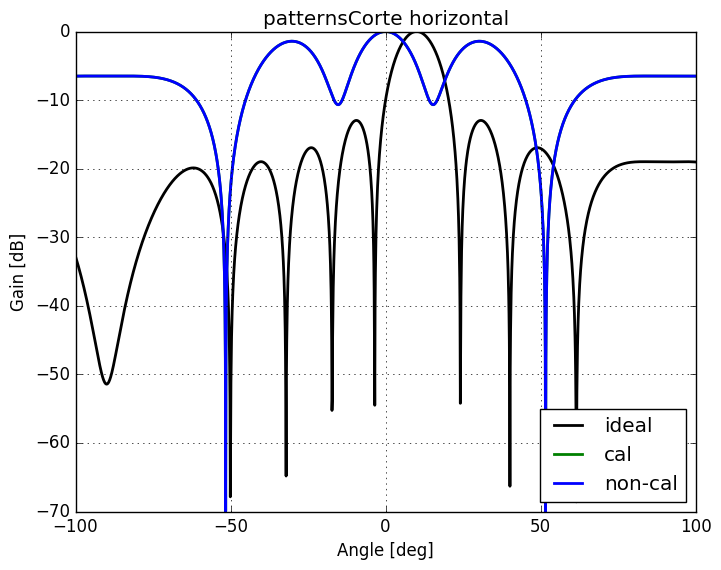
\includegraphics[width=7cm]{gfx/deadTRMsMutual10degColAzCut.png}}
	\subfloat[Corte en rango (vertical) del diagrama de radiación]{
		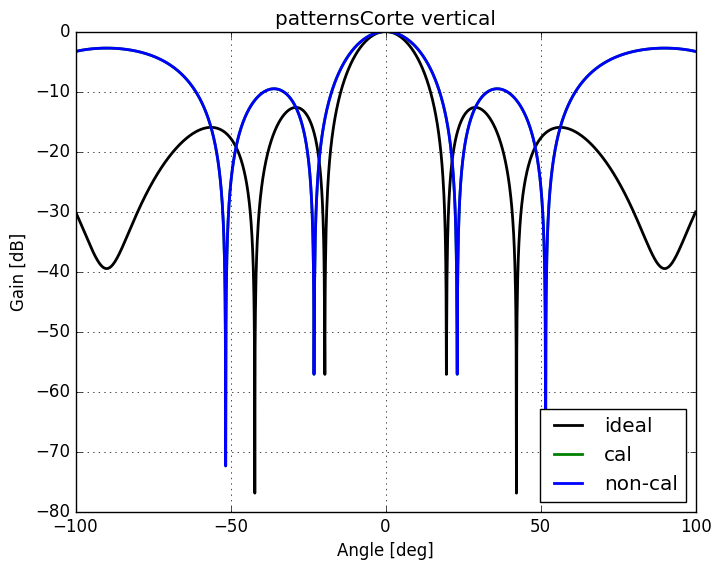
\includegraphics[width=7cm]{gfx/deadTRMsMutual10degColElCut.png}}
	\caption{Señales transmitidas por la antena en los casos deseado (ideal), pre (non-cal) y post (cal) calibración por acoplamientos mutuos.}
	\label{fig:deadTRMsMutual10degCol}
\end{figure}
La tabla \ref{tab:deadTRMsMutual10degCol} muestra que las diferencias de ganancia de los lóbulos secundarios entre los 
diagramas de radiación reales y el ideal para el corte horizontal es de -0.2 dB, el signo negativo indica que el lóbulo del
diagrama calibrado es mayor que el ideal. En el corte vertical dicha diferencia es de -1.03 dB, la cual resulta un incremento
inadmisible. A su vez, se puede apreciar que la diferencia en la ganancia del lóbulo principal en ambos cortes disminuyó en
0.39 dB y 0.82 dB respectivamente. Por último, el ancho del lóbulo principal de la señal calibrada es igual al ideal. 
\begin{table}[H]
  \footnotesize
  \centering
  \begin{tabular}{|c|c|C{2cm}|C{2.5cm}|C{2.5cm}|C{2.5cm}|}
    \hline
    Caso & Corte & Ganancia - lóbulo izq. [dBc] & Ganancia - lóbulo central [dB] &
    Ganancia - lóbulo der. [dBc] & Ancho - lóbulo central -3dB \tabularnewline\hline
    \multirow{2}{2cm}{Diag. rad. sin calibrar} & H & 12.31 & 43.1 & 12.31 & 12.4 \tabularnewline\cline{2-6}
     & V & 11.87 & 33.06 & 12.13 & 17.2 \tabularnewline\hline
    \multirow{2}{2cm}{Diag. rad. calibrado} & H & 12.77 & 42.51 & 11.88 & 12.4 \tabularnewline\cline{2-6}
     & V & 11.62 & 32.14 & 11.84 & 17.4 \tabularnewline\hline
    \multirow{2}{2cm}{Diag. rad. ideal} & H & 12.97 & 42.9 & 12.97 & 12.4 \tabularnewline\cline{2-6}
     & V & 12.65 & 32.96 & 12.65 & 17.4 \tabularnewline\hline
    \multirow{2}{2cm}{Dif. sin calibrar} & H & -0.66 & 0.2 & -0.66 & 0.0\tabularnewline\cline{2-6}
     & V & -0.78 & 0.1 & -0.52 & -0.2 \tabularnewline\hline
    \multirow{2}{2cm}{Dif. calibrado} & H & -0.2 & -0.39 & -1.09 & 0.0 \tabularnewline\cline{2-6}
     & V & -1.03 & -0.82 & -0.81 & 0.0 \tabularnewline\hline
  \end{tabular}
  \caption{Propiedades de los diagramas de radiación calibrados y sin calibrar comparados con el ideal.}
  \label{tab:deadTRMsMutual10degCol}
\end{table}


\subsubsection{Apuntamiento 10 grados en rango (vertical)}

En la figuras \ref{fig:nonErrMutual10degRow} se puede verificar que el apuntamiento es el correcto por los desfases observados, 
como hay 10 elementos radiantes por fila, al apuntar verticalmente, cada fila posee un desfase diferente, es por esta razón que 
la tercer fila se ve un gráfico estilo una escalera con siete escalones (que es la cantidad de columnas de la antena). A su vez, 
se aprecia que el calibrador lleva tanto la potencia como la fase transmitida al valor deseado.

Analizando los diagramas de radiación, se observa que debido a la causa de TRMs dañados, se aprecia un aumento considerable de
ambos lóbulos secundarios del corte horizontal, generando así que la diferencia con el lóbulo principal sea menor. En el corte
vertical no se aprecia tal diferencia. 

Los tres estados de señales graficados son el deseado (caso ideal), el previo a calibrar (non-cal) y el resultante de la
calibración (cal).
\begin{figure}[H]
	\centering
 	\subfloat[Ganancia y fase transmitida por cada ER]{
		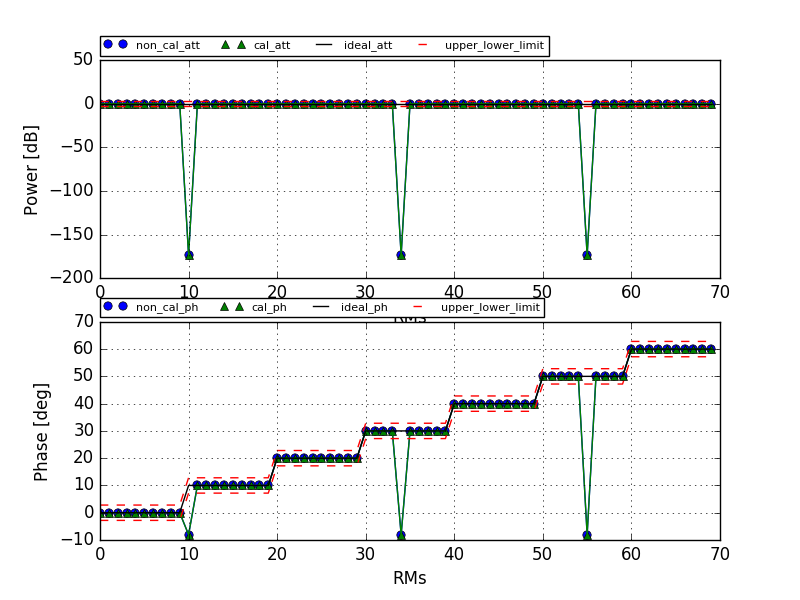
\includegraphics[width=9cm]{gfx/deadTRMsMutual10degRow.png}}

	\subfloat[Corte en azimut (horizontal) del diagrama de radiación]{
		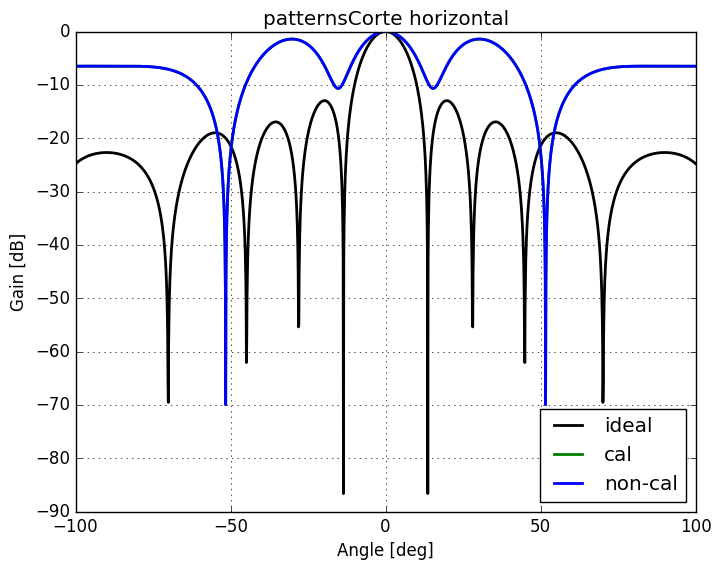
\includegraphics[width=7cm]{gfx/deadTRMsMutual10degRowAzCut.png}}
	\subfloat[Corte en rango (vertical) del diagrama de radiación]{
		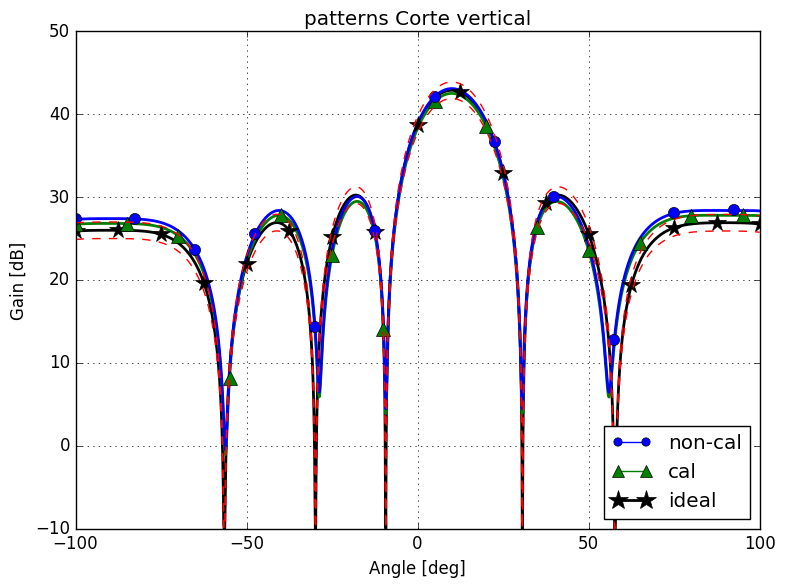
\includegraphics[width=7cm]{gfx/deadTRMsMutual10degRowElCut.png}}
	\caption{Señales transmitidas por la antena en los casos deseado (ideal), pre (non-cal) y post (cal) calibración por acoplamientos mutuos.}
	\label{fig:deadTRMsMutual10degRow}
\end{figure}
La tabla \ref{tab:deadTRMsMutual10degRow} muestra que las diferencias de ganancia de los lóbulos secundarios entre los 
diagramas de radiación reales y el ideal para el corte horizontal es de -1.41 dB (dicho valor es mayor que el admisible, 1 dB),
el signo negativo indica que la ganancia del lóbulo del diagrama calibrado es mayor que el ideal. En el corte vertical dicha
diferencia es de 0.38 dB. A su vez, se puede apreciar que las ganancias de los lóbulos principales de los cortes horizontales y
verticales son menores al ideal en 0.43 dB y 0.38 dB respectivamente. Por último, el ancho de los lóbulos principales no resultan
afectados. 
\begin{table}[H]
  \footnotesize
  \centering
  \begin{tabular}{|c|c|C{2cm}|C{2.5cm}|C{2.5cm}|C{2.5cm}|}
    \hline
    Caso & Corte & Ganancia - lóbulo izq. [dBc] & Ganancia - lóbulo central [dB] &
    Ganancia - lóbulo der. [dBc] & Ancho - lóbulo central -3dB \tabularnewline\hline
    \multirow{2}{2cm}{Diag. rad. sin calibrar} & H & 11.56 & 38.91 & 12.75 & 12.0 \tabularnewline\cline{2-6}
     & V & 13.03 & 43.1 & 13.03 & 17.8 \tabularnewline\hline
    \multirow{2}{2cm}{Diag. rad. calibrado} & H & 11.56 & 38.33 & 12.75 & 12.0 \tabularnewline\cline{2-6}
     & V & 13.03 & 42.52 & 13.03 & 17.8 \tabularnewline\hline
    \multirow{2}{2cm}{Diag. rad. ideal} & H & 12.97 & 38.76 & 12.97 & 12.0 \tabularnewline\cline{2-6}
     & V & 12.65 & 42.9 & 12.65 & 17.8 \tabularnewline\hline
    \multirow{2}{2cm}{Dif. sin calibrar} & H & -1.41 & 0.15 & -0.22 & 0.0\tabularnewline\cline{2-6}
     & V & 0.38 & 0.2 & 0.38 & 0.0 \tabularnewline\hline
    \multirow{2}{2cm}{Dif. calibrado} & H & -1.41 & -0.43 & -0.22 & 0.0 \tabularnewline\cline{2-6}
     & V & 0.38 & -0.38 & 0.38 & 0.0 \tabularnewline\hline
  \end{tabular}
  \caption{Propiedades de los diagramas de radiación calibrados y sin calibrar comparados con el ideal.}
  \label{tab:deadTRMsMutual10degRow}
\end{table}


\section{Dispersiones en comportamiento de componentes de la antena}
\label{sc:withDispersion} 

Los casos de simulación de esta sección tienen las siguientes características,
\begin{itemize}
	\item Hay dispersiones de comportamiento en los siguientes componentes de la antena: circuladores, TRMs, PSCs y RMs. Las 
		magnitudes están especificadas en la tabla \ref{tab:errorReferences}.
		\begin{table}[H]
		  \footnotesize
		  \centering
		  \begin{tabular}{|c|c|}
			\hline
			\textbf{Dispersiones de componente} & \textbf{Desvío estandar} \tabularnewline \hline 
			Ganancia del circulador &  0.2 [dB] \tabularnewline\hline 
			Fase del circulador &  10 [deg] \tabularnewline\hline 
			Ganancia del TRM &  0.2 [dB] \tabularnewline\hline 
			Fase del TRM &  10 [deg] \tabularnewline\hline 
			Ganancia del PSC &  0.1 [dB] \tabularnewline\hline 
			Fase del PSC &  10 [deg] \tabularnewline\hline 
		  \end{tabular}
		  \caption{Configuración de los errores de componentes.}
		  \label{tab:errorReferences}
		\end{table}
	\item No hay TRMs dañados.
	\item No hay dispersiones en la señal, la misma es invariante en el tiempo.
\end{itemize}

\subsection{Calibración clásica con dispersiones en la respuesta de componentes}
\label{ssc:classicalDispersion}

A continuación se presentan los tres casos de prueba definidos en la sección \ref{sc:characteristics} para el método de
calibración interna clásico.


\subsubsection{Apuntamiento uniforme}

Los gráficos de la figura \ref{fig:compErrClassical0deg} muestran que el calibrador ya comienza a mostrar sus falencias no 
logrando calibrar completamente la señal transmitida. Comparando la ganancia y fase de cada ER calibrado con respecto a los
valores ideales, se aprecia una diferencia máxima de 5 dB y 70 grados respectivamente.

Analizando los diagramas de radiación, se observa que si bien el diagrama calibrado resulta parecido al ideal, presenta ganancias
de lóbulos secundarios mayores a los deseados.

Los tres estados de señales graficados son el deseado (caso ideal), el previo a calibrar (non-cal) y el resultante de la
calibración (cal).
\begin{figure}[H]
	\centering
 	\subfloat[Ganancia y fase transmitida por cada ER]{
		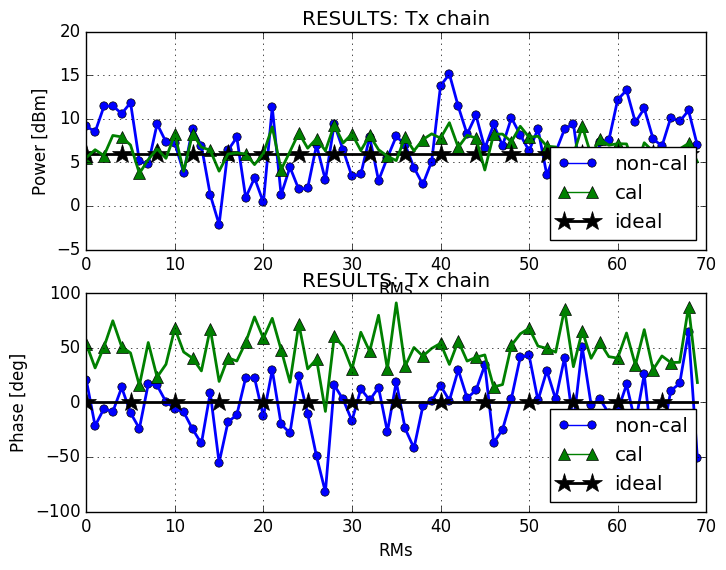
\includegraphics[width=9cm]{gfx/compErrClassical0deg.png}}

	\subfloat[Corte en azimut (horizontal) del diagrama de radiación]{
		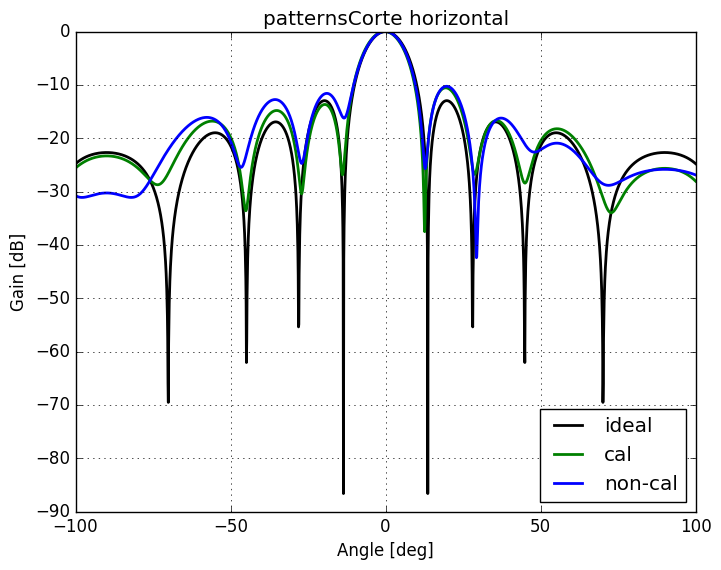
\includegraphics[width=7cm]{gfx/compErrClassical0degAzCut.png}}
	\subfloat[Corte en rango (vertical) del diagrama de radiación]{
		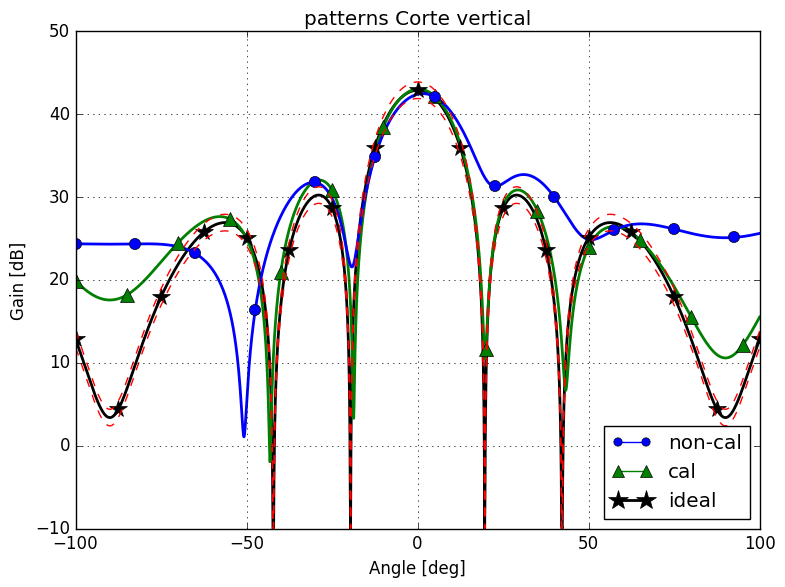
\includegraphics[width=7cm]{gfx/compErrClassical0degElCut.png}}
	\caption{señal transmitida utilizando calibración clásica. (a) ganancia y fase transmitida. (b) corte horizontal del 
	diagrama de radiación y (c) corte vertical del diagrama de radiación.}
	\label{fig:compErrClassical0deg}
\end{figure}
La tabla \ref{tab:compErrClassical0deg} muestra que las diferencias de ganancia de los lóbulos secundarios entre los diagramas 
reales y el ideal para el corte vertical es de -1.66 dBc (valor que supera el límite admisible de -1 dBc). El signo negativo
indica que el lóbulo del diagrama calibrado es mayor que el ideal. En el corte vertical dicha diferencia es casi la mitad, de
-0.75 dBc. A su vez, se puede apreciar que la diferencia en la ganancia del lóbulo principal se disminuyó a los 0.15 dB y que el
ancho del mismo en el corte vertical es 0.2 grados menor.

\begin{table}[H]
  \footnotesize
  \centering
  \begin{tabular}{|c|c|C{2cm}|C{2.5cm}|C{2.5cm}|C{2.5cm}|}
    \hline
    Caso & Corte & Ganancia - lóbulo izq. [dBc] & Ganancia - lóbulo central [dB] &
    Ganancia - lóbulo der. [dBc] & Ancho - lóbulo central -3dB \tabularnewline\hline
    \multirow{2}{2cm}{Diag. rad. sin calibrar} & H & 11.15 & 42.42 & 15.66 & 12.2 \tabularnewline\cline{2-6}
     & V & 10.71 & 42.49 & 9.77 & 19.4 \tabularnewline\hline
    \multirow{2}{2cm}{Diag. rad. calibrado} & H & 12.22 & 43.05 & 12.93 & 12.0 \tabularnewline\cline{2-6}
     & V & 10.99 & 43.05 & 12.19 & 17.2 \tabularnewline\hline
    \multirow{2}{2cm}{Diag. rad. ideal} & H & 12.97 & 42.9 & 12.97 & 12.0 \tabularnewline\cline{2-6}
     & V & 12.65 & 42.9 & 12.65 & 17.4 \tabularnewline\hline
    \multirow{2}{2cm}{Dif. sin calibrar} & H & -1.82 & -0.48 & 2.69 & 0.2\tabularnewline\cline{2-6}
     & V & -1.94 & -0.41 & -2.88 & 2.0 \tabularnewline\hline
    \multirow{2}{2cm}{Dif. calibrado} & H & -0.75 & 0.15 & -0.04 & 0.0 \tabularnewline\cline{2-6}
     & V & -1.66 & 0.15 & -0.46 & -0.2 \tabularnewline\hline
  \end{tabular}
  \caption{Propiedades de los diagramas de radiación calibrados y sin calibrar comparados con el ideal.}
  \label{tab:compErrClassical0deg}
\end{table}


\subsubsection{Apuntamiento 10 grados en azimut (horizontal)}

Los gráficos de la figura \ref{fig:compErrClassical10degCol} muestran que el calibrador ya comienza a mostrar sus falencias no 
logrando calibrar completamente la señal transmitida. Comparando la ganancia y fase de cada ER calibrado con respecto a los
valores ideales, se aprecia una diferencia máxima de 5 dB y 50 grados respectivamente.

Analizando los diagramas de radiación, se observa que si bien el diagrama calibrado en el corte horizontal resulta parecido al
ideal, presenta ganancias de lóbulos secundarios mayores a los deseados. El diagrama del corte posee el lóbulo principal más
ancho que el ideal.

Los tres estados de señales graficados son el deseado (caso ideal), el previo a calibrar (non-cal) y el resultante de la
calibración (cal).
\begin{figure}[H]
	\centering
 	\subfloat[Ganancia y fase transmitida por cada ER]{
		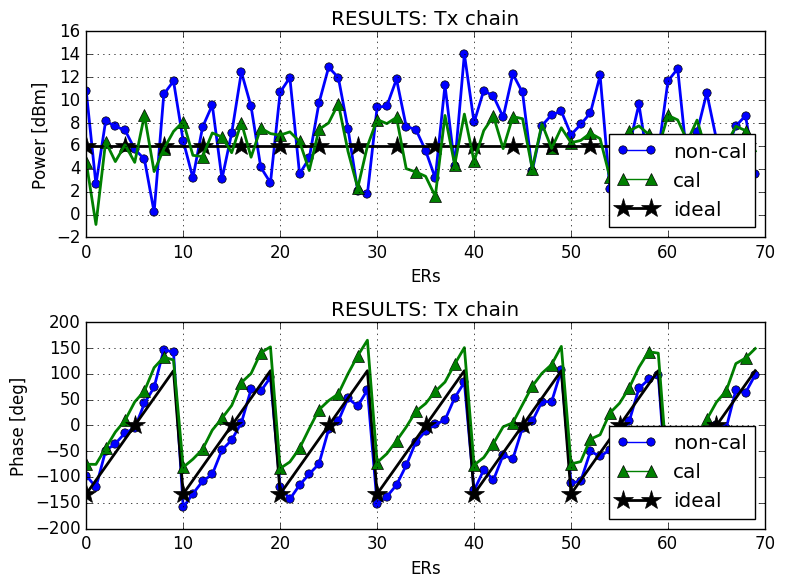
\includegraphics[width=9cm]{gfx/compErrClassical10degCol.png}}

	\subfloat[Corte en azimut (horizontal) del diagrama de radiación]{
		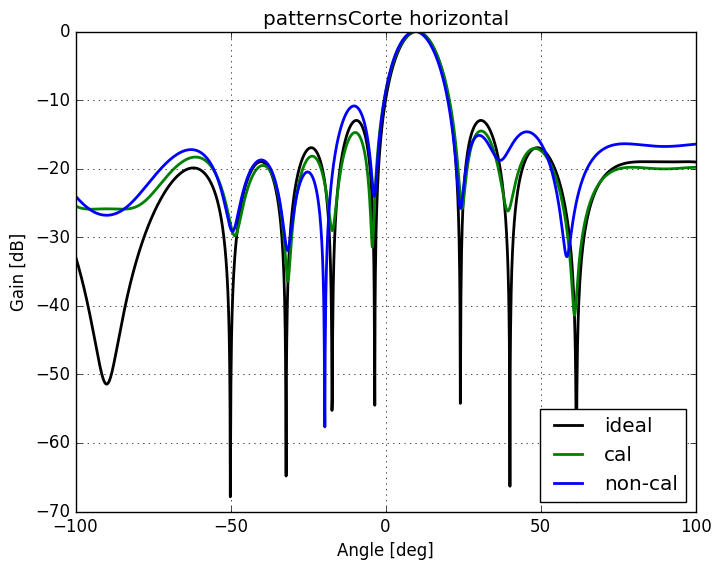
\includegraphics[width=7cm]{gfx/compErrClassical10degColAzCut.png}}
	\subfloat[Corte en rango (vertical) del diagrama de radiación]{
		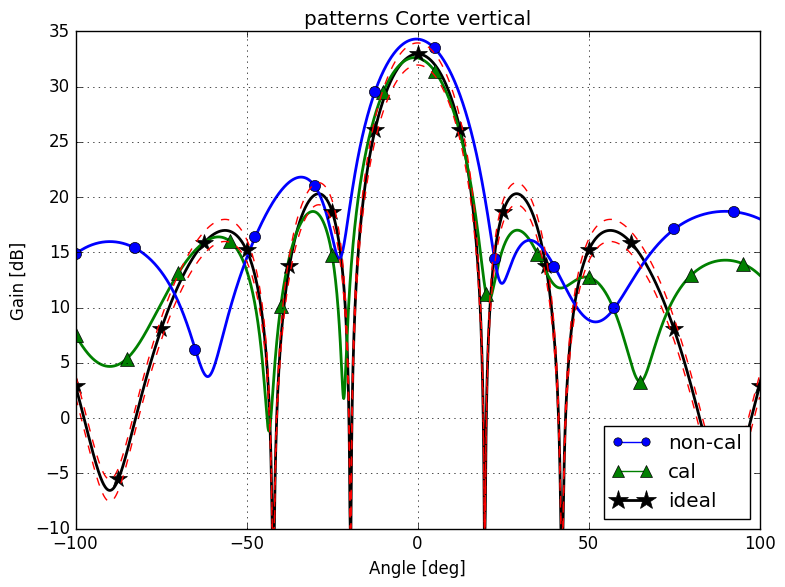
\includegraphics[width=7cm]{gfx/compErrClassical10degColElCut.png}}
	\caption{señal transmitida utilizando calibración clásica. (a) ganancia y fase transmitida. (b) corte horizontal del 
	diagrama de radiación y (c) corte vertical del diagrama de radiación.}
	\label{fig:compErrClassical10degCol}
\end{figure}
La tabla \ref{tab:compErrClassical10degCol} muestra que las diferencias de ganancia de los lóbulos secundarios entre los diagramas 
reales y el ideal para el corte vertical es de -1.41 dBc (valor que supera el límite admisible de -1 dBc). El signo negativo
indica que el lóbulo del diagrama calibrado es mayor que el ideal. En el corte vertical dicha diferencia es de 1.28 dBc. A su
vez, se puede apreciar que la diferencia en la ganancia del lóbulo principal se disminuyó a los 0.35 dB y que el ancho del mismo
en el corte vertical es de 1 grado mayor.

\begin{table}[H]
  \footnotesize
  \centering
  \begin{tabular}{|c|c|C{2cm}|C{2.5cm}|C{2.5cm}|C{2.5cm}|}
    \hline
    Caso & Corte & Ganancia - lóbulo izq. [dBc] & Ganancia - lóbulo central [dB] &
    Ganancia - lóbulo der. [dBc] & Ancho - lóbulo central -3dB \tabularnewline\hline
    \multirow{2}{2cm}{Diag. rad. sin calibrar} & H & 12.19 & 44.36 & 14.67 & 12.6 \tabularnewline\cline{2-6}
     & V & 12.5 & 34.31 & 18.21 & 20.0 \tabularnewline\hline
    \multirow{2}{2cm}{Diag. rad. calibrado} & H & 11.56 & 43.25 & 13.35 & 12.4 \tabularnewline\cline{2-6}
     & V & 13.93 & 32.63 & 15.62 & 18.4 \tabularnewline\hline
    \multirow{2}{2cm}{Diag. rad. ideal} & H & 12.97 & 42.9 & 12.97 & 12.4 \tabularnewline\cline{2-6}
     & V & 12.65 & 32.96 & 12.65 & 17.4 \tabularnewline\hline
    \multirow{2}{2cm}{Dif. sin calibrar} & H & -0.78 & 1.46 & 1.7 & 0.2\tabularnewline\cline{2-6}
     & V & -0.15 & 1.35 & 5.56 & 2.6 \tabularnewline\hline
    \multirow{2}{2cm}{Dif. calibrado} & H & -1.41 & 0.35 & 0.38 & 0.0 \tabularnewline\cline{2-6}
     & V & 1.28 & -0.33 & 2.97 & 1.0 \tabularnewline\hline
  \end{tabular}
  \caption{Propiedades de los diagramas de radiación calibrados y sin calibrar comparados con el ideal.}
  \label{tab:compErrClassical10degCol}
\end{table}


\subsubsection{Apuntamiento 10 grados en rango (vertical)}

Los gráficos de la figura \ref{fig:compErrClassical10degRow} muestran que el calibrador ya comienza a mostrar sus falencias no 
logrando calibrar completamente la señal transmitida. Comparando la ganancia y fase de cada ER calibrado con respecto a los
valores ideales, se aprecia una diferencia máxima de 5 dB y 50 grados respectivamente.

Analizando los diagramas de radiación, se observa que si bien los diagramas calibrados en el corte horizontal y vertical
resultan parecidos al ideal, presentan ganancias de lóbulos secundarios mayores a los deseados. 

Los tres estados de señales graficados son el deseado (caso ideal), el previo a calibrar (non-cal) y el resultante de la
calibración (cal).
\begin{figure}[H]
	\centering
 	\subfloat[Ganancia y fase transmitida por cada ER]{
		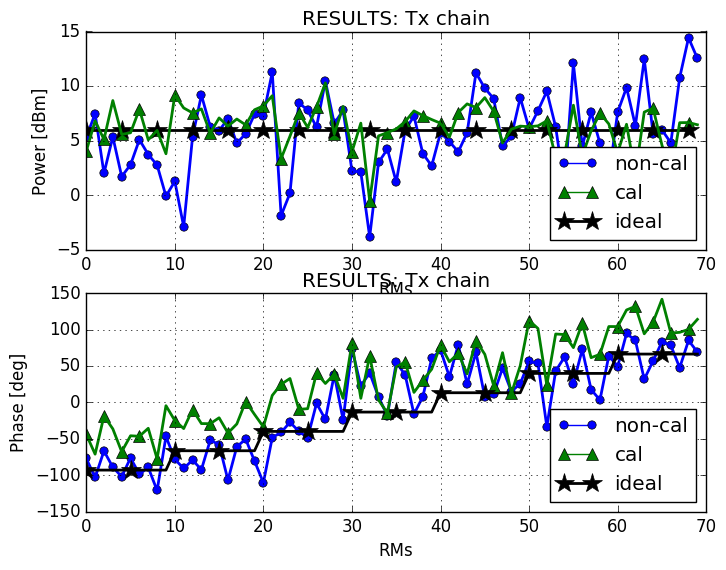
\includegraphics[width=9cm]{gfx/compErrClassical10degRow.png}}

	\subfloat[Corte en azimut (horizontal) del diagrama de radiación]{
		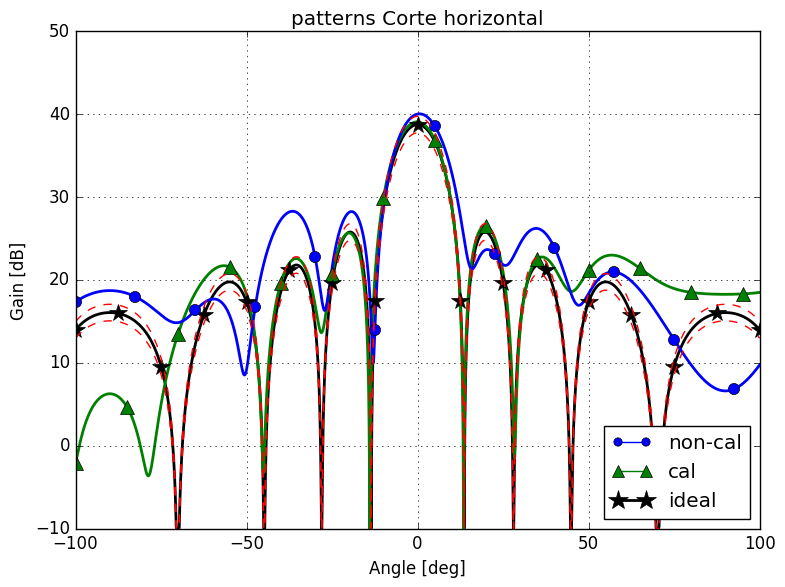
\includegraphics[width=7cm]{gfx/compErrClassical10degRowAzCut.png}}
	\subfloat[Corte en rango (vertical) del diagrama de radiación]{
		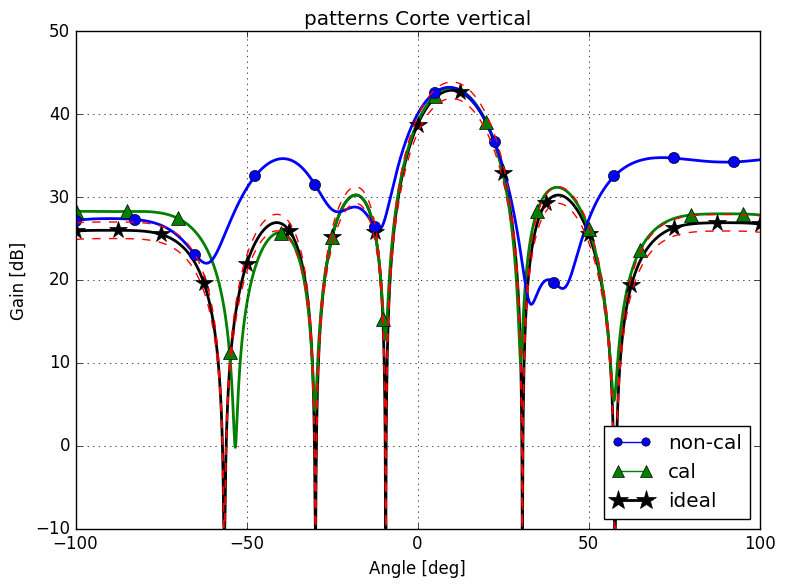
\includegraphics[width=7cm]{gfx/compErrClassical10degRowElCut.png}}
	\caption{señal transmitida utilizando calibración clásica. (a) ganancia y fase transmitida. (b) corte horizontal del 
	diagrama de radiación y (c) corte vertical del diagrama de radiación.}
	\label{fig:compErrClassical10degRow}
\end{figure}
La tabla \ref{tab:compErrClassical10degCol} muestra que las diferencias de ganancia de los lóbulos secundarios entre los diagramas 
reales y el ideal para el corte vertical es de -0.41 dBc. El signo negativo indica que el lóbulo del diagrama calibrado es mayor
que el ideal. En el corte vertical dicha diferencia es de -0.67 dBc. A su vez, se puede apreciar que la diferencia en la ganancia
del lóbulo principal se incrementó en 0.33 dB y que el ancho del mismo en el corte vertical es de 0.2 grados menor y el del corte
horizontal 0.2 grados mayor.
\begin{table}[H]
  \footnotesize
  \centering
  \begin{tabular}{|c|c|C{2cm}|C{2.5cm}|C{2.5cm}|C{2.5cm}|}
    \hline
    Caso & Corte & Ganancia - lóbulo izq. [dBc] & Ganancia - lóbulo central [dB] &
    Ganancia - lóbulo der. [dBc] & Ancho - lóbulo central -3dB \tabularnewline\hline
    \multirow{2}{2cm}{Diag. rad. sin calibrar} & H & 11.8 & 40.05 & 16.38 & 12.6 \tabularnewline\cline{2-6}
     & V & 14.45 & 43.26 & 23.23 & 18.6 \tabularnewline\hline
    \multirow{2}{2cm}{Diag. rad. calibrado} & H & 13.41 & 39.09 & 12.56 & 12.2 \tabularnewline\cline{2-6}
     & V & 12.9 & 43.16 & 11.98 & 17.6 \tabularnewline\hline
    \multirow{2}{2cm}{Diag. rad. ideal} & H & 12.97 & 38.76 & 12.97 & 12.0 \tabularnewline\cline{2-6}
     & V & 12.65 & 42.9 & 12.65 & 17.8 \tabularnewline\hline
    \multirow{2}{2cm}{Dif. sin calibrar} & H & -1.17 & 1.29 & 3.41 & 0.6\tabularnewline\cline{2-6}
     & V & 1.8 & 0.36 & 10.58 & 0.8 \tabularnewline\hline
    \multirow{2}{2cm}{Dif. calibrado} & H & 0.44 & 0.33 & -0.41 & 0.2 \tabularnewline\cline{2-6}
     & V & 0.25 & 0.26 & -0.67 & -0.2 \tabularnewline\hline
  \end{tabular}
  \caption{Propiedades de los diagramas de radiación calibrados y sin calibrar comparados con el ideal.}
  \label{tab:compErrClassical10degRow}
\end{table}


\subsection{Calibración por acoplamientos mutuos con dispersiones en la respuesta de componentes}

A continuación se presentan los tres casos de prueba definidos en la sección \ref{sc:characteristics} para el método de
calibración por acoplamientos mutuos.


\subsubsection{Apuntamiento uniforme}

Los gráficos de la figura \ref{fig:compErrMutual0deg} muestran que el calibrador funciona correctamente y que los diagramas de 
radiación de la señal calibrada se asemejan al ideal. 

Analizando los diagramas de radiación, se observa que los diagramas de radiación calibrados resultan semejantes a los deseados. 

Los tres estados de señales graficados son el deseado (caso ideal), el previo a calibrar (non-cal) y el resultante de la
calibración (cal).
\begin{figure}[H]
	\centering
 	\subfloat[Ganancia y fase transmitida por cada ER]{
		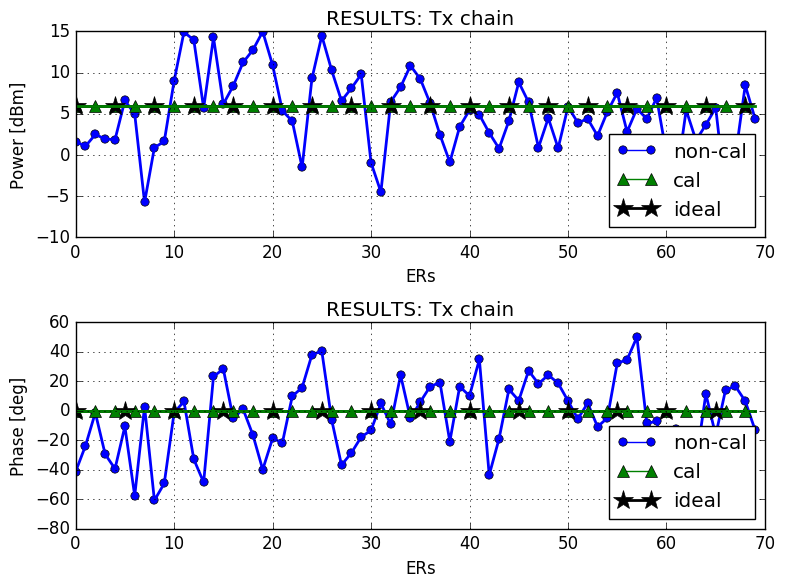
\includegraphics[width=9cm]{gfx/compErrMutual0deg.png}}

	\subfloat[Corte en azimut (horizontal) del diagrama de radiación]{
		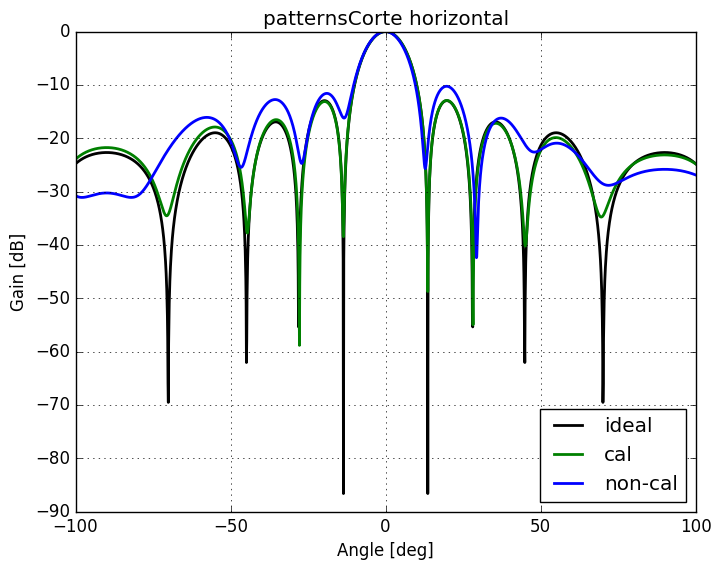
\includegraphics[width=7cm]{gfx/compErrMutual0degAzCut.png}}
	\subfloat[Corte en rango (vertical) del diagrama de radiación]{
		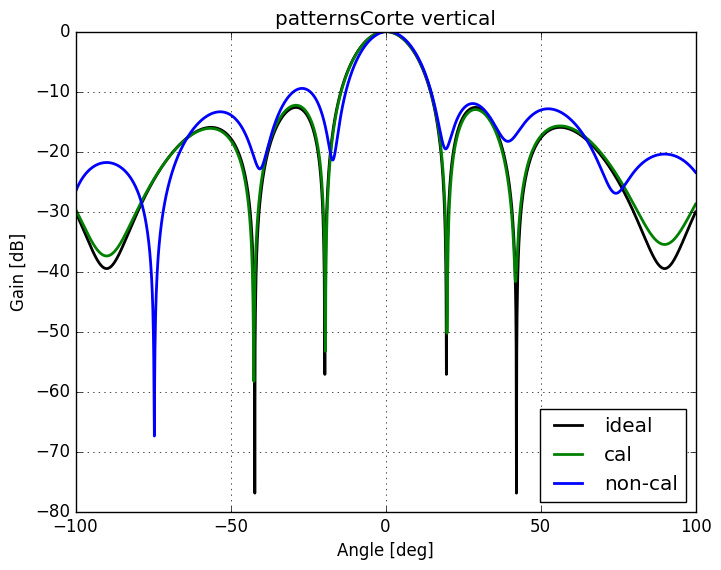
\includegraphics[width=7cm]{gfx/compErrMutual0degElCut.png}}
	\caption{señal transmitida calibrada por acoplamientos mutuos. (a) ganancia y fase transmitida. (b) corte horizontal del 
	diagrama de radiación y (c) corte vertical del diagrama de radiación.}
	\label{fig:compErrMutual0deg}
\end{figure}

La tabla \ref{tab:compErrMutual0deg} muestra que las diferencias de ganancia de los lóbulos secundarios entre los diagramas 
reales y el ideal para ambos cortes son iguales a cero. A su vez, se observa que la ganancia y el ancho de los lóbulos
principales son iguales a los deseados.

\begin{table}[H]
  \footnotesize
  \centering
  \begin{tabular}{|c|c|C{2cm}|C{2.5cm}|C{2.5cm}|C{2.5cm}|}
    \hline
    Caso & Corte & Ganancia - lóbulo izq. [dBc] & Ganancia - lóbulo central [dB] &
    Ganancia - lóbulo der. [dBc] & Ancho - lóbulo central -3dB \tabularnewline\hline
    \multirow{2}{2cm}{Diag. rad. sin calibrar} & H & 11.15 & 42.42 & 15.66 & 12.2 \tabularnewline\cline{2-6}
     & V & 10.71 & 42.49 & 9.77 & 19.4 \tabularnewline\hline
    \multirow{2}{2cm}{Diag. rad. calibrado} & H & 12.97 & 42.9 & 12.97 & 12.0 \tabularnewline\cline{2-6}
     & V & 12.65 & 42.9 & 12.65 & 17.4 \tabularnewline\hline
    \multirow{2}{2cm}{Diag. rad. ideal} & H & 12.97 & 42.9 & 12.97 & 12.0 \tabularnewline\cline{2-6}
     & V & 12.65 & 42.9 & 12.65 & 17.4 \tabularnewline\hline
    \multirow{2}{2cm}{Dif. sin calibrar} & H & -1.82 & -0.48 & 2.69 & 0.2\tabularnewline\cline{2-6}
     & V & -1.94 & -0.41 & -2.88 & 2.0 \tabularnewline\hline
    \multirow{2}{2cm}{Dif. calibrado} & H & 0.0 & 0.0 & 0.0 & 0.0 \tabularnewline\cline{2-6}
     & V & 0.0 & 0.0 & 0.0 & 0.0 \tabularnewline\hline
  \end{tabular}
  \caption{Propiedades de los diagramas de radiación calibrados y sin calibrar comparados con el ideal.}
  \label{tab:compErrMutual0deg}
\end{table}


\subsubsection{Apuntamiento 10 grados en azimut (horizontal)}

Los gráficos de la figura \ref{fig:compErrMutual10degCol} muestran que el calibrador funciona correctamente y que los diagramas de 
radiación de la señal calibrada se asemejan al ideal. 

Analizando los diagramas de radiación, se observa que los diagramas de radiación calibrados resultan semejantes a los deseados. 

Los tres estados de señales graficados son el deseado (caso ideal), el previo a calibrar (non-cal) y el resultante de la
calibración (cal).
\begin{figure}[H]
	\centering
 	\subfloat[Ganancia y fase transmitida por cada ER]{
		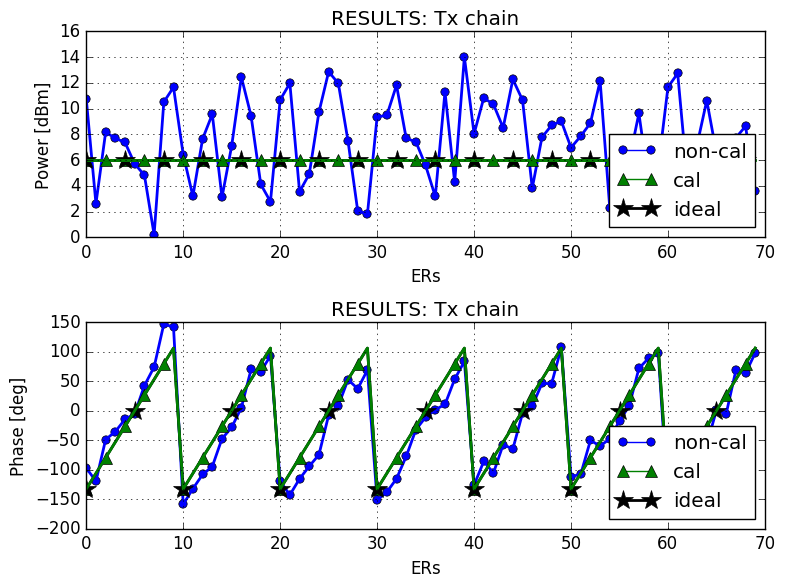
\includegraphics[width=9cm]{gfx/compErrMutual10degCol.png}}

	\subfloat[Corte en azimut (horizontal) del diagrama de radiación]{
		\includegraphics[width=7cm]{gfx/compErrMutual10degColAzCut.png}}
	\subfloat[Corte en rango (vertical) del diagrama de radiación]{
		\includegraphics[width=7cm]{gfx/compErrMutual10degColElCut.png}}
	\caption{señal transmitida calibrada por acoplamientos mutuos. (a) ganancia y fase transmitida. (b) corte horizontal del 
	diagrama de radiación y (c) corte vertical del diagrama de radiación.}
	\label{fig:compErrMutual10degCol}
\end{figure}

La tabla \ref{tab:compErrMutual10degCol} muestra que las diferencias de ganancia de los lóbulos secundarios entre los diagramas 
reales y el ideal para ambos cortes son iguales a cero. A su vez, se observa que la ganancia y el ancho de los lóbulos
principales son iguales a los deseados.

\begin{table}[H]
  \footnotesize
  \centering
  \begin{tabular}{|c|c|C{2cm}|C{2.5cm}|C{2.5cm}|C{2.5cm}|}
    \hline
    Caso & Corte & Ganancia - lóbulo izq. [dBc] & Ganancia - lóbulo central [dB] &
    Ganancia - lóbulo der. [dBc] & Ancho - lóbulo central -3dB \tabularnewline\hline
    \multirow{2}{2cm}{Diag. rad. sin calibrar} & H & 12.19 & 44.36 & 14.67 & 12.6 \tabularnewline\cline{2-6}
     & V & 12.5 & 34.31 & 18.21 & 20.0 \tabularnewline\hline
    \multirow{2}{2cm}{Diag. rad. calibrado} & H & 12.97 & 42.9 & 12.97 & 12.4 \tabularnewline\cline{2-6}
     & V & 12.65 & 32.96 & 12.65 & 17.4 \tabularnewline\hline
    \multirow{2}{2cm}{Diag. rad. ideal} & H & 12.97 & 42.9 & 12.97 & 12.4 \tabularnewline\cline{2-6}
     & V & 12.65 & 32.96 & 12.65 & 17.4 \tabularnewline\hline
    \multirow{2}{2cm}{Dif. sin calibrar} & H & -0.78 & 1.46 & 1.7 & 0.2\tabularnewline\cline{2-6}
     & V & -0.15 & 1.35 & 5.56 & 2.6 \tabularnewline\hline
    \multirow{2}{2cm}{Dif. calibrado} & H & 0.0 & 0.0 & 0.0 & 0.0 \tabularnewline\cline{2-6}
     & V & 0.0 & 0.0 & 0.0 & 0.0 \tabularnewline\hline
  \end{tabular}
  \caption{Propiedades de los diagramas de radiación calibrados y sin calibrar comparados con el ideal.}
  \label{tab:compErrMutual10degCol}
\end{table}


\subsubsection{Apuntamiento 10 grados en rango (vertical)}

Los gráficos de la figura \ref{fig:compErrMutual10degRow} muestran que el calibrador funciona correctamente y que los diagramas de 
radiación de la señal calibrada se asemejan al ideal. 

Analizando los diagramas de radiación, se observa que los diagramas de radiación calibrados resultan semejantes a los deseados. 

Los tres estados de señales graficados son el deseado (caso ideal), el previo a calibrar (non-cal) y el resultante de la
calibración (cal).
\begin{figure}[H]
	\centering
 	\subfloat[Ganancia y fase transmitida por cada ER]{
		\includegraphics[width=9cm]{gfx/compErrMutual10degRow.png}}

	\subfloat[Corte en azimut (horizontal) del diagrama de radiación]{
		\includegraphics[width=7cm]{gfx/compErrMutual10degRowAzCut.png}}
	\subfloat[Corte en rango (vertical) del diagrama de radiación]{
		\includegraphics[width=7cm]{gfx/compErrMutual10degRowElCut.png}}
	\caption{señal transmitida calibrada por acoplamientos mutuos. (a) ganancia y fase transmitida. (b) corte horizontal del 
	diagrama de radiación y (c) corte vertical del diagrama de radiación.}
	\label{fig:compErrMutual10degRow}
\end{figure}

La tabla \ref{tab:compErrMutual10degRow} muestra que las diferencias de ganancia de los lóbulos secundarios entre los diagramas 
reales y el ideal presentan una diferencia de -0.07 dBc para el corte horizontal y 0.01 para el corte vertical. A su vez, se
observa que la ganancia y el ancho de los lóbulos principales son iguales a los deseados.

\begin{table}[H]
  \footnotesize
  \centering
  \begin{tabular}{|c|c|C{2cm}|C{2.5cm}|C{2.5cm}|C{2.5cm}|}
    \hline
    Caso & Corte & Ganancia - lóbulo izq. [dBc] & Ganancia - lóbulo central [dB] &
    Ganancia - lóbulo der. [dBc] & Ancho - lóbulo central -3dB \tabularnewline\hline
    \multirow{2}{2cm}{Diag. rad. sin calibrar} & H & 11.8 & 40.05 & 16.38 & 12.6 \tabularnewline\cline{2-6}
     & V & 14.45 & 43.26 & 23.23 & 18.6 \tabularnewline\hline
    \multirow{2}{2cm}{Diag. rad. calibrado} & H & 12.9 & 38.75 & 12.91 & 12.0 \tabularnewline\cline{2-6}
     & V & 12.66 & 42.9 & 12.66 & 17.8 \tabularnewline\hline
    \multirow{2}{2cm}{Diag. rad. ideal} & H & 12.97 & 38.76 & 12.97 & 12.0 \tabularnewline\cline{2-6}
     & V & 12.65 & 42.9 & 12.65 & 17.8 \tabularnewline\hline
    \multirow{2}{2cm}{Dif. sin calibrar} & H & -1.17 & 1.29 & 3.41 & 0.6\tabularnewline\cline{2-6}
     & V & 1.8 & 0.36 & 10.58 & 0.8 \tabularnewline\hline
    \multirow{2}{2cm}{Dif. calibrado} & H & -0.07 & -0.01 & -0.06 & 0.0 \tabularnewline\cline{2-6}
     & V & 0.01 & 0.0 & 0.01 & 0.0 \tabularnewline\hline
  \end{tabular}
  \caption{Propiedades de los diagramas de radiación calibrados y sin calibrar comparados con el ideal.}
  \label{tab:compErrMutual10degRow}
\end{table}


\section{Dispersiones de ganancia entre pulsos}
\label{sc:withPulsesGainDispersion}

En esta sección se agregan dispersiones de fase y ganancia en el generador de la señal utilizada para transmitir y calibrar 
la antena. Las otras características de este ensayo son:
\begin{itemize}
	\item Desvío estándar en ganancia de 1 dB entre pulsos de calibración.
	\item Desvío estándar en fase de 5 grados entre pulsos de calibración.
	\item No hay dispersiones en el comportamiento de los componentes de la antena.
	\item No hay TRMs dañados.
\end{itemize}

\subsection{Calibración clásica con dispersiones de ganancia entre pulsos}

A continuación se presentan los tres casos de prueba definidos en la sección \ref{sc:characteristics} para el método de
calibración interna clásico.


\subsubsection{Apuntamiento uniforme}

En las imágenes de la figura \ref{fig:chirpErrClassical0deg} se puede apreciar como, sacando de lado la diferencia de 
ganancia y fase por no abarcar la completitud del sistema, esta incertidumbre hace que el calibrador no funcione correctamente 
ni para medir fase ni ganancias de cada elemento, introduciendo diferencias de hasta 8 dBs en ganancia y 48 grados en fase.
A su vez, se puede observar que los diagramas de radiación poseen una gran diferencia en ganancia.

Los tres estados de señales graficados son el deseado (caso ideal), el previo a calibrar (non-cal) y el resultante de la
calibración (cal).
\begin{figure}[H]
	\centering
 	\subfloat[Ganancia y fase transmitida por cada ER]{
		\includegraphics[width=9cm]{gfx/chirpErrClassical0deg.png}}

	\subfloat[Corte en azimut (horizontal) del diagrama de radiación]{
		\includegraphics[width=7cm]{gfx/chirpErrClassical0degAzCut.png}}
	\subfloat[Corte en rango (vertical) del diagrama de radiación]{
		\includegraphics[width=7cm]{gfx/chirpErrClassical0degElCut.png}}
	\caption{Señales transmitidas por la antena en los casos deseado (ideal), pre (non-cal) y post (cal) calibración clásica.}
	\label{fig:chirpErrClassical0deg}
\end{figure}

En la tabla \ref{tab:chirpErrClassical0deg} se pueden apreciar que si bien las ganancias de los lóbulos principales son muy 
diferentes, rondando los 2.4 dBs, los diagramas de radiación poseen lóbulos secundarios mayores al ideal por medio dBc. El 
ancho del lóbulo principal también se ve afectado, resultando en 0.6 grados mayor para el corte vertical.

\begin{table}[H]
  \footnotesize
  \centering
  \begin{tabular}{|c|c|C{2cm}|C{2.5cm}|C{2.5cm}|C{2.5cm}|}
    \hline
    Caso & Corte & Ganancia - lóbulo izq. [dBc] & Ganancia - lóbulo central [dB] &
    Ganancia - lóbulo der. [dBc] & Ancho - lóbulo central -3dB \tabularnewline\hline
    \multirow{2}{2cm}{Diag. rad. sin calibrar} & H & 12.97 & 43.48 & 12.97 & 12.0 \tabularnewline\cline{2-6}
     & V & 12.65 & 43.48 & 12.65 & 17.4 \tabularnewline\hline
    \multirow{2}{2cm}{Diag. rad. calibrado} & H & 12.39 & 45.04 & 12.51 & 12.0 \tabularnewline\cline{2-6}
     & V & 13.85 & 45.04 & 12.87 & 18.0 \tabularnewline\hline
    \multirow{2}{2cm}{Diag. rad. ideal} & H & 12.97 & 42.9 & 12.97 & 12.0 \tabularnewline\cline{2-6}
     & V & 12.65 & 42.9 & 12.65 & 17.4 \tabularnewline\hline
    \multirow{2}{2cm}{Dif. sin calibrar} & H & 0.0 & 0.58 & 0.0 & 0.0\tabularnewline\cline{2-6}
     & V & 0.0 & 0.58 & 0.0 & 0.0 \tabularnewline\hline
    \multirow{2}{2cm}{Dif. calibrado} & H & -0.58 & 2.14 & -0.46 & 0.0 \tabularnewline\cline{2-6}
     & V & 1.2 & 2.14 & 0.22 & 0.6 \tabularnewline\hline
  \end{tabular}
  \caption{Propiedades de los diagramas de radiación calibrados y sin calibrar comparados con el ideal.}
  \label{tab:chirpErrClassical0deg}
\end{table}


\subsubsection{Apuntamiento 10 grados en azimut (horizontal)}

En las imágenes de la figura \ref{fig:chirpErrClassical10degCol} se puede apreciar como, sacando de lado la diferencia de 
ganancia y fase por no abarcar la completitud del sistema, esta incertidumbre hace que el calibrador no funcione correctamente 
ni para medir fase ni ganancias de cada elemento, introduciendo diferencias de hasta 14 dBs en ganancia y 200 grados en fase. 
A su vez, se puede observar que los diagramas de radiación poseen lóbulos secundarios con una ganancia mucho mayor a la aceptada.

Los tres estados de señales graficados son el deseado (caso ideal), el previo a calibrar (non-cal) y el resultante de la
calibración (cal).
\begin{figure}[H]
	\centering
 	\subfloat[Ganancia y fase transmitida por cada ER]{
		\includegraphics[width=9cm]{gfx/chirpErrClassical10degCol.png}}

	\subfloat[Corte en azimut (horizontal) del diagrama de radiación]{
		\includegraphics[width=7cm]{gfx/chirpErrClassical10degColAzCut.png}}
	\subfloat[Corte en rango (vertical) del diagrama de radiación]{
		\includegraphics[width=7cm]{gfx/chirpErrClassical10degColElCut.png}}
	\caption{señal transmitida utilizando calibración clásica. (a) ganancia y fase transmitida. (b) corte horizontal del 
	diagrama de radiación y (c) corte vertical del diagrama de radiación.}
	\label{fig:chirpErrClassical10degCol}
\end{figure}

En la tabla \ref{tab:chirpErrClassical10degCol} se pueden apreciar que si bien las ganancias de los lóbulos principales son 
diferentes por 9.2 dBs, las diferencias por los lóbulos secundarios rondan los .-2 dBc, valor que supera ampliamente el límite
admisible de -1dBc. El ancho del lóbulo principal también se ve afectado, resultando en aproximadamente 0.8 grados mayor para el
corte horizontal.

\begin{table}[H]
  \footnotesize
  \centering
  \begin{tabular}{|c|c|C{2cm}|C{2.5cm}|C{2.5cm}|C{2.5cm}|}
    \hline
    Caso & Corte & Ganancia - lóbulo izq. [dBc] & Ganancia - lóbulo central [dB] &
    Ganancia - lóbulo der. [dBc] & Ancho - lóbulo central -3dB \tabularnewline\hline
    \multirow{2}{2cm}{Diag. rad. sin calibrar} & H & 12.97 & 43.48 & 12.97 & 12.4 \tabularnewline\cline{2-6}
     & V & 12.65 & 33.54 & 12.65 & 17.4 \tabularnewline\hline
    \multirow{2}{2cm}{Diag. rad. calibrado} & H & 15.08 & 52.16 & 14.82 & 13.2 \tabularnewline\cline{2-6}
     & V & 10.63 & 41.23 & 11.58 & 16.0 \tabularnewline\hline
    \multirow{2}{2cm}{Diag. rad. ideal} & H & 12.97 & 42.9 & 12.97 & 12.4 \tabularnewline\cline{2-6}
     & V & 12.65 & 32.96 & 12.65 & 17.4 \tabularnewline\hline
    \multirow{2}{2cm}{Dif. sin calibrar} & H & 0.0 & 0.58 & 0.0 & 0.0\tabularnewline\cline{2-6}
     & V & 0.0 & 0.58 & 0.0 & 0.0 \tabularnewline\hline
    \multirow{2}{2cm}{Dif. calibrado} & H & 2.11 & 9.26 & 1.85 & 0.8 \tabularnewline\cline{2-6}
     & V & -2.02 & 8.27 & -1.07 & -1.4 \tabularnewline\hline
  \end{tabular}
  \caption{Propiedades de los diagramas de radiación calibrados y sin calibrar comparados con el ideal.}
  \label{tab:chirpErrClassical10degCol}
\end{table}


\subsubsection{Apuntamiento 10 grados en rango (vertical)}

En las imágenes de la figura \ref{fig:chirpErrClassical10degRow} se puede apreciar como, sacando de lado la diferencia de 
ganancia y fase por no abarcar la completitud del sistema, esta incertidumbre hace que el calibrador no funcione correctamente 
ni para medir fase ni ganancias de cada elemento, introduciendo diferencias de hasta 15 dBs en ganancia y 100 grados en fase. 
A su vez, se puede observar que los diagramas de radiación poseen lóbulos secundarios con una ganancia mucho mayor a la aceptada.

Los tres estados de señales graficados son el deseado (caso ideal), el previo a calibrar (non-cal) y el resultante de la
calibración (cal).
\begin{figure}[H]
	\centering
 	\subfloat[Ganancia y fase transmitida por cada ER]{
		\includegraphics[width=9cm]{gfx/chirpErrClassical10degRow.png}}

	\subfloat[Corte en azimut (horizontal) del diagrama de radiación]{
		\includegraphics[width=7cm]{gfx/chirpErrClassical10degRowAzCut.png}}
	\subfloat[Corte en rango (vertical) del diagrama de radiación]{
		\includegraphics[width=7cm]{gfx/chirpErrClassical10degRowElCut.png}}
	\caption{señal transmitida utilizando calibración clásica. (a) ganancia y fase transmitida. (b) corte horizontal del 
	diagrama de radiación y (c) corte vertical del diagrama de radiación.}
	\label{fig:chirpErrClassical10degRow}
\end{figure}

En la tabla \ref{tab:chirpErrClassical10degRow} se pueden apreciar que si bien las ganancias de los lóbulos principales son 
diferentes por 14.26 dBs, las diferencias por los lóbulos secundarios rondan los -6.73 dBc, valor que supera ampliamente el
máximo permitido de -1dBc. El ancho del lóbulo principal también se ve afectado, resultando en aproximadamente -1.2 grados
menor.

\begin{table}[H]
  \footnotesize
  \centering
  \begin{tabular}{|c|c|C{2cm}|C{2.5cm}|C{2.5cm}|C{2.5cm}|}
    \hline
    Caso & Corte & Ganancia - lóbulo izq. [dBc] & Ganancia - lóbulo central [dB] &
    Ganancia - lóbulo der. [dBc] & Ancho - lóbulo central -3dB \tabularnewline\hline
    \multirow{2}{2cm}{Diag. rad. sin calibrar} & H & 12.97 & 39.34 & 12.97 & 12.0 \tabularnewline\cline{2-6}
     & V & 12.65 & 43.48 & 12.65 & 17.8 \tabularnewline\hline
    \multirow{2}{2cm}{Diag. rad. calibrado} & H & 12.14 & 53.02 & 11.03 & 11.8 \tabularnewline\cline{2-6}
     & V & 16.73 & 54.3 & 5.92 & 16.6 \tabularnewline\hline
    \multirow{2}{2cm}{Diag. rad. ideal} & H & 12.97 & 38.76 & 12.97 & 12.0 \tabularnewline\cline{2-6}
     & V & 12.65 & 42.9 & 12.65 & 17.8 \tabularnewline\hline
    \multirow{2}{2cm}{Dif. sin calibrar} & H & 0.0 & 0.58 & 0.0 & 0.0\tabularnewline\cline{2-6}
     & V & 0.0 & 0.58 & 0.0 & 0.0 \tabularnewline\hline
    \multirow{2}{2cm}{Dif. calibrado} & H & -0.83 & 14.26 & -1.94 & -0.2 \tabularnewline\cline{2-6}
     & V & 4.08 & 11.4 & -6.73 & -1.2 \tabularnewline\hline
  \end{tabular}
  \caption{Propiedades de los diagramas de radiación calibrados y sin calibrar comparados con el ideal.}
  \label{tab:chirpErrClassical10degRow}
\end{table}


\subsection{Calibración por acoplamientos mutuos con dispersiones de ganancia entre pulsos}

A continuación se presentan los tres casos de prueba definidos en la sección \ref{sc:characteristics} para el método de
calibración por acoplamientos mutuos.


\subsubsection{Apuntamiento uniforme}

En las imágenes de la figura \ref{fig:chirpErrMutual0deg} se puede apreciar como esta incertidumbre hace que el calibrador 
no funcione tan correctamente ni para medir fase ni ganancias de cada elemento, introduciendo diferencias de hasta 1 dB en 
ganancia y -14 grados en fase. A su vez, se puede observar que, independientemente de este desvío introducido, los diagramas de 
radiación se mantienen cerca del esperado, salvo por la ganancia esperada.

Los tres estados de señales graficados son el deseado (caso ideal), el previo a calibrar (non-cal) y el resultante de la
calibración (cal).
\begin{figure}[H]
	\centering
 	\subfloat[Ganancia y fase transmitida por cada ER]{
		\includegraphics[width=9cm]{gfx/chirpErrMutual0deg.png}}

	\subfloat[Corte en azimut (horizontal) del diagrama de radiación]{
		\includegraphics[width=7cm]{gfx/chirpErrMutual0degAzCut.png}}
	\subfloat[Corte en rango (vertical) del diagrama de radiación]{
		\includegraphics[width=7cm]{gfx/chirpErrMutual0degElCut.png}}
	\caption{Señales transmitidas por la antena en los casos deseado (ideal), pre (non-cal) y post (cal) calibración por acoplamientos mutuos.}
	\label{fig:chirpErrMutual0deg}
\end{figure}

En la tabla \ref{tab:chirpErrMutual0deg} se pueden apreciar que si bien las ganancias de los lóbulos principales son 
diferentes por 0.1 dBs, las diferencias por los lóbulos secundarios rondan los -0.04 dBc. Se puede concluir que el 
calibrador es bastante robusto frente a esta clase de incertidumbres. El ancho del lóbulo principal también se ve afectado,
resultando en 0.2 grados mayor para el corte horizontal.

\begin{table}[H]
  \footnotesize
  \centering
  \begin{tabular}{|c|c|C{2cm}|C{2.5cm}|C{2.5cm}|C{2.5cm}|}
    \hline
    Caso & Corte & Ganancia - lóbulo izq. [dBc] & Ganancia - lóbulo central [dB] &
    Ganancia - lóbulo der. [dBc] & Ancho - lóbulo central -3dB \tabularnewline\hline
    \multirow{2}{2cm}{Diag. rad. sin calibrar} & H & 12.97 & 43.48 & 12.97 & 12.0 \tabularnewline\cline{2-6}
     & V & 12.65 & 43.48 & 12.65 & 17.4 \tabularnewline\hline
    \multirow{2}{2cm}{Diag. rad. calibrado} & H & 13.13 & 43.0 & 13.02 & 12.2 \tabularnewline\cline{2-6}
     & V & 12.61 & 43.0 & 12.76 & 17.4 \tabularnewline\hline
    \multirow{2}{2cm}{Diag. rad. ideal} & H & 12.97 & 42.9 & 12.97 & 12.0 \tabularnewline\cline{2-6}
     & V & 12.65 & 42.9 & 12.65 & 17.4 \tabularnewline\hline
    \multirow{2}{2cm}{Dif. sin calibrar} & H & 0.0 & 0.58 & 0.0 & 0.0\tabularnewline\cline{2-6}
     & V & 0.0 & 0.58 & 0.0 & 0.0 \tabularnewline\hline
    \multirow{2}{2cm}{Dif. calibrado} & H & 0.16 & 0.1 & 0.05 & 0.2 \tabularnewline\cline{2-6}
     & V & -0.04 & 0.1 & 0.11 & 0.0 \tabularnewline\hline
  \end{tabular}
  \caption{Propiedades de los diagramas de radiación calibrados y sin calibrar comparados con el ideal.}
  \label{tab:chirpErrMutual0deg}
\end{table}


\subsubsection{Apuntamiento 10 grados en azimut (horizontal)}

En las imágenes de la figura \ref{fig:chirpErrMutual10degCol} se puede apreciar como esta incertidumbre hace que el calibrador 
no funcione tan correctamente ni para medir fase ni ganancias de cada elemento, introduciendo diferencias de hasta 0.9 dBs en 
ganancia y unos pocos grados en fase. A su vez, se puede observar que, independientemente de este desvío introducido, los
diagramas de radiación se mantienen cerca del esperado.

Los tres estados de señales graficados son el deseado (caso ideal), el previo a calibrar (non-cal) y el resultante de la
calibración (cal).
\begin{figure}[H]
	\centering
 	\subfloat[Ganancia y fase transmitida por cada ER]{
		\includegraphics[width=9cm]{gfx/chirpErrMutual10degCol.png}}

	\subfloat[Corte en azimut (horizontal) del diagrama de radiación]{
		\includegraphics[width=7cm]{gfx/chirpErrMutual10degColAzCut.png}}
	\subfloat[Corte en rango (vertical) del diagrama de radiación]{
		\includegraphics[width=7cm]{gfx/chirpErrMutual10degColElCut.png}}
	\caption{Señales transmitidas por la antena en los casos deseado (ideal), pre (non-cal) y post (cal) calibración por acoplamientos mutuos.}
	\label{fig:chirpErrMutual10degCol}
\end{figure}

En la tabla \ref{tab:chirpErrMutual10degCol} se pueden apreciar que las ganancias de los lóbulos principales es mayor a la
deseada por 0.3 dB y que los peores casos de los lóbulos principales son de -0.07 dBc para el corte horizontal y -0.18 para el
corte vertical. Se puede concluir que el calibrador es bastante robusto frente a esta clase de incertidumbres. El ancho del
lóbulo principal también se ve afectado, resultando en aproximadamente 0.2 grados menor para el corte vertical.

\begin{table}[H]
  \footnotesize
  \centering
  \begin{tabular}{|c|c|C{2cm}|C{2.5cm}|C{2.5cm}|C{2.5cm}|}
    \hline
    Caso & Corte & Ganancia - lóbulo izq. [dBc] & Ganancia - lóbulo central [dB] &
    Ganancia - lóbulo der. [dBc] & Ancho - lóbulo central -3dB \tabularnewline\hline
    \multirow{2}{2cm}{Diag. rad. sin calibrar} & H & 12.97 & 43.48 & 12.97 & 12.4 \tabularnewline\cline{2-6}
     & V & 12.65 & 33.54 & 12.65 & 17.4 \tabularnewline\hline
    \multirow{2}{2cm}{Diag. rad. calibrado} & H & 12.9 & 43.19 & 13.07 & 12.4 \tabularnewline\cline{2-6}
     & V & 13.18 & 33.28 & 12.47 & 17.2 \tabularnewline\hline
    \multirow{2}{2cm}{Diag. rad. ideal} & H & 12.97 & 42.9 & 12.97 & 12.4 \tabularnewline\cline{2-6}
     & V & 12.65 & 32.96 & 12.65 & 17.4 \tabularnewline\hline
    \multirow{2}{2cm}{Dif. sin calibrar} & H & 0.0 & 0.58 & 0.0 & 0.0\tabularnewline\cline{2-6}
     & V & 0.0 & 0.58 & 0.0 & 0.0 \tabularnewline\hline
    \multirow{2}{2cm}{Dif. calibrado} & H & -0.07 & 0.29 & 0.1 & 0.0 \tabularnewline\cline{2-6}
     & V & 0.53 & 0.32 & -0.18 & -0.2 \tabularnewline\hline
  \end{tabular}
  \caption{Propiedades de los diagramas de radiación calibrados y sin calibrar comparados con el ideal.}
  \label{tab:chirpErrMutual10degCol}
\end{table}


\subsubsection{Apuntamiento 10 grados en rango (vertical)}

En las imágenes de la figura \ref{fig:chirpErrMutual10degRow} se puede apreciar cómo esta incertidumbre hace que el calibrador 
no funcione tan correctamente ni para medir fase ni ganancias de cada elemento, introduciendo diferencias de hasta 2.5 dBs en 
ganancia y unos 10 grados en fase. A su vez, se puede observar que, independientemente de este desvío introducido, los diagramas
de radiación se mantienen cerca del esperado, salvo por la ganancia de los mismos.

Los tres estados de señales graficados son el deseado (caso ideal), el previo a calibrar (non-cal) y el resultante de la
calibración (cal).
\begin{figure}[H]
	\centering
 	\subfloat[Ganancia y fase transmitida por cada ER]{
		\includegraphics[width=9cm]{gfx/chirpErrMutual10degRow.png}}

	\subfloat[Corte en azimut (horizontal) del diagrama de radiación]{
		\includegraphics[width=7cm]{gfx/chirpErrMutual10degRowAzCut.png}}
	\subfloat[Corte en rango (vertical) del diagrama de radiación]{
		\includegraphics[width=7cm]{gfx/chirpErrMutual10degRowElCut.png}}
	\caption{Señales transmitidas por la antena en los casos deseado (ideal), pre (non-cal) y post (cal) calibración por acoplamientos mutuos.}
	\label{fig:chirpErrMutual10degRow}
\end{figure}

En la tabla \ref{tab:chirpErrMutual10degRow} se pueden apreciar que las ganancias de los lóbulos principales resultan ser menores
a las esperadas por 1.3 dBs y que el peor caso de diferencia de los lóbulos secundarios es de -0.12 dBc para el corte horizontal.
Se puede concluir que el calibrador es bastante robusto frente a esta clase de incertidumbres. El ancho del lóbulo principal
también se ve afectado, resultando en aproximadamente 0.2 grados mayor para el corte horizontal.

\begin{table}[H]
  \footnotesize
  \centering
  \begin{tabular}{|c|c|C{2cm}|C{2.5cm}|C{2.5cm}|C{2.5cm}|}
    \hline
    Caso & Corte & Ganancia - lóbulo izq. [dBc] & Ganancia - lóbulo central [dB] &
    Ganancia - lóbulo der. [dBc] & Ancho - lóbulo central -3dB \tabularnewline\hline
    \multirow{2}{2cm}{Diag. rad. sin calibrar} & H & 12.97 & 39.34 & 12.97 & 12.0 \tabularnewline\cline{2-6}
     & V & 12.65 & 43.48 & 12.65 & 17.8 \tabularnewline\hline
    \multirow{2}{2cm}{Diag. rad. calibrado} & H & 12.85 & 37.4 & 13.64 & 12.2 \tabularnewline\cline{2-6}
     & V & 12.72 & 41.51 & 12.67 & 17.8 \tabularnewline\hline
    \multirow{2}{2cm}{Diag. rad. ideal} & H & 12.97 & 38.76 & 12.97 & 12.0 \tabularnewline\cline{2-6}
     & V & 12.65 & 42.9 & 12.65 & 17.8 \tabularnewline\hline
    \multirow{2}{2cm}{Dif. sin calibrar} & H & 0.0 & 0.58 & 0.0 & 0.0\tabularnewline\cline{2-6}
     & V & 0.0 & 0.58 & 0.0 & 0.0 \tabularnewline\hline
    \multirow{2}{2cm}{Dif. calibrado} & H & -0.12 & -1.36 & 0.67 & 0.2 \tabularnewline\cline{2-6}
     & V & 0.07 & -1.39 & 0.02 & 0.0 \tabularnewline\hline
  \end{tabular}
  \caption{Propiedades de los diagramas de radiación calibrados y sin calibrar comparados con el ideal.}
  \label{tab:chirpErrMutual10degRow}
\end{table}


\section{Dispersión de ganancia de la chirp réplica}
\label{sc:withChirpPulsesGainDispersion}

Como la chirp réplica es solamente utilizada en la calibración clásica, en esta simulación no se podrán comparar 
resultados, pero sirve para determinar que tan robusto es el método para esta clase de errores. Por como funciona el método, 
se espera un desfase en la caracterización igual para todos los elementos tanto en ganancia como en fase. El desvío estándar
utilizado es de 1dB para la ganancia y 5 grados para la fase.

Los tres casos de prueba presentados en las siguientes secciones poseen las características definidas en la sección
\ref{sc:characteristics}.


\subsection{Apuntamiento uniforme}

En las imágenes de la figura \ref{fig:chirpRepErrClassical0deg} se puede apreciar como, sacando de lado la diferencia de 
ganancia y fase por no abarcar la completitud del sistema, la ganancia calibrada de cada elemento radiante resulta en 6 dB
por debajo de la esperada y sus fases poseen una diferencia de 50 grados a la esperada. De todas formas, es importante resaltar
que el diagrama de radiación no resulta deformado. 

Los tres estados de señales graficados son el deseado (caso ideal), el previo a calibrar (non-cal) y el resultante de la
calibración (cal).

\begin{figure}[H]
	\centering
 	\subfloat[Ganancia y fase transmitida por cada ER]{
		\includegraphics[width=9cm]{gfx/chirpRepErrClassical0deg.png}}

	\subfloat[Corte en azimut (horizontal) del diagrama de radiación]{
		\includegraphics[width=7cm]{gfx/chirpRepErrClassical0degAzCut.png}}
	\subfloat[Corte en rango (vertical) del diagrama de radiación]{
		\includegraphics[width=7cm]{gfx/chirpRepErrClassical0degElCut.png}}
	\caption{Señales transmitidas por la antena en los casos deseado (ideal), pre (non-cal) y post (cal) calibración clásica.}
	\label{fig:chirpRepErrClassical0deg}
\end{figure}

En la tabla \ref{tab:chirpRepErrClassical0deg} se pueden apreciar que no hay diferencias en los lóbulos secundarios ni en el
ancho del lóbulo principal. Si es apreciable la diferencia en ganancia de todo el diagrama de radiación, el cual es de 6.1 dB
menor al esperado.

\begin{table}[H]
  \footnotesize
  \centering
  \begin{tabular}{|c|c|C{2cm}|C{2.5cm}|C{2.5cm}|C{2.5cm}|}
    \hline
    Caso & Corte & Ganancia - lóbulo izq. [dBc] & Ganancia - lóbulo central [dB] &
    Ganancia - lóbulo der. [dBc] & Ancho - lóbulo central -3dB \tabularnewline\hline
    \multirow{2}{2cm}{Diag. rad. sin calibrar} & H & 12.97 & 43.48 & 12.97 & 12.0 \tabularnewline\cline{2-6}
     & V & 12.65 & 43.48 & 12.65 & 17.4 \tabularnewline\hline
    \multirow{2}{2cm}{Diag. rad. calibrado} & H & 12.97 & 36.8 & 12.97 & 12.0 \tabularnewline\cline{2-6}
     & V & 12.65 & 36.8 & 12.65 & 17.4 \tabularnewline\hline
    \multirow{2}{2cm}{Diag. rad. ideal} & H & 12.97 & 42.9 & 12.97 & 12.0 \tabularnewline\cline{2-6}
     & V & 12.65 & 42.9 & 12.65 & 17.4 \tabularnewline\hline
    \multirow{2}{2cm}{Dif. sin calibrar} & H & 0.0 & 0.58 & 0.0 & 0.0\tabularnewline\cline{2-6}
     & V & 0.0 & 0.58 & 0.0 & 0.0 \tabularnewline\hline
    \multirow{2}{2cm}{Dif. calibrado} & H & 0.0 & -6.1 & 0.0 & 0.0 \tabularnewline\cline{2-6}
     & V & 0.0 & -6.1 & 0.0 & 0.0 \tabularnewline\hline
  \end{tabular}
  \caption{Propiedades de los diagramas de radiación calibrados y sin calibrar comparados con el ideal.}
  \label{tab:chirpRepErrClassical0deg}
\end{table}


\subsection{Apuntamiento 10 grados en azimut (horizontal)}

En las imágenes de la figura \ref{fig:chirpRepErrClassical10degCol} se puede apreciar como, sacando de lado la diferencia de 
ganancia y fase por no abarcar la completitud del sistema, la ganancia calibrada de cada elemento radiante resulta en 6 dB
por debajo de la esperada y sus fases poseen una diferencia de 50 grados a la esperada. De todas formas, es importante resaltar
que el diagrama de radiación no resulta deformado. 

Los tres estados de señales graficados son el deseado (caso ideal), el previo a calibrar (non-cal) y el resultante de la
calibración (cal).

\begin{figure}[H]
	\centering
 	\subfloat[Ganancia y fase transmitida por cada ER]{
		\includegraphics[width=9cm]{gfx/chirpRepErrClassical10degCol.png}}

	\subfloat[Corte en azimut (horizontal) del diagrama de radiación]{
		\includegraphics[width=7cm]{gfx/chirpRepErrClassical10degColAzCut.png}}
	\subfloat[Corte en rango (vertical) del diagrama de radiación]{
		\includegraphics[width=7cm]{gfx/chirpRepErrClassical10degColElCut.png}}
	\caption{Señales transmitidas por la antena en los casos deseado (ideal), pre (non-cal) y post (cal) calibración clásica.}
	\label{fig:chirpRepErrClassical10degCol}
\end{figure}

En la tabla \ref{tab:chirpRepErrClassical10degCol} se pueden apreciar que no hay diferencias en los lóbulos secundarios ni en el
ancho del lóbulo principal. Si es apreciable la diferencia en ganancia de todo el diagrama de radiación, el cual es de 6.1 dB
menor al esperado.

\begin{table}[H]
  \footnotesize
  \centering
  \begin{tabular}{|c|c|C{2cm}|C{2.5cm}|C{2.5cm}|C{2.5cm}|}
    \hline
    Caso & Corte & Ganancia - lóbulo izq. [dBc] & Ganancia - lóbulo central [dB] &
    Ganancia - lóbulo der. [dBc] & Ancho - lóbulo central -3dB \tabularnewline\hline
    \multirow{2}{2cm}{Diag. rad. sin calibrar} & H & 12.97 & 43.48 & 12.97 & 12.4 \tabularnewline\cline{2-6}
     & V & 12.65 & 33.54 & 12.65 & 17.4 \tabularnewline\hline
    \multirow{2}{2cm}{Diag. rad. calibrado} & H & 12.97 & 36.8 & 12.97 & 12.4 \tabularnewline\cline{2-6}
     & V & 12.65 & 26.86 & 12.65 & 17.4 \tabularnewline\hline
    \multirow{2}{2cm}{Diag. rad. ideal} & H & 12.97 & 42.9 & 12.97 & 12.4 \tabularnewline\cline{2-6}
     & V & 12.65 & 32.96 & 12.65 & 17.4 \tabularnewline\hline
    \multirow{2}{2cm}{Dif. sin calibrar} & H & 0.0 & 0.58 & 0.0 & 0.0\tabularnewline\cline{2-6}
     & V & 0.0 & 0.58 & 0.0 & 0.0 \tabularnewline\hline
    \multirow{2}{2cm}{Dif. calibrado} & H & 0.0 & -6.1 & 0.0 & 0.0 \tabularnewline\cline{2-6}
     & V & 0.0 & -6.1 & 0.0 & 0.0 \tabularnewline\hline
  \end{tabular}
  \caption{Propiedades de los diagramas de radiación calibrados y sin calibrar comparados con el ideal.}
  \label{tab:chirpRepErrClassical10degCol}
\end{table}


\subsection{Apuntamiento 10 grados en rango (vertical)}

En las imágenes de la figura \ref{fig:chirpRepErrClassical10degRow} se puede apreciar como, sacando de lado la diferencia de 
ganancia y fase por no abarcar la completitud del sistema, la ganancia calibrada de cada elemento radiante resulta en 6 dB
por debajo de la esperada y sus fases poseen una diferencia de 50 grados a la esperada. De todas formas, es importante resaltar
que el diagrama de radiación no resulta deformado. 

Los tres estados de señales graficados son el deseado (caso ideal), el previo a calibrar (non-cal) y el resultante de la
calibración (cal).

\begin{figure}[H]
	\centering
 	\subfloat[Ganancia y fase transmitida por cada ER]{
		\includegraphics[width=9cm]{gfx/chirpRepErrClassical10degRow.png}}

	\subfloat[Corte en azimut (horizontal) del diagrama de radiación]{
		\includegraphics[width=7cm]{gfx/chirpRepErrClassical10degRowAzCut.png}}
	\subfloat[Corte en rango (vertical) del diagrama de radiación]{
		\includegraphics[width=7cm]{gfx/chirpRepErrClassical10degRowElCut.png}}
	\caption{Señales transmitidas por la antena en los casos deseado (ideal), pre (non-cal) y post (cal) calibración clásica.}
	\label{fig:chirpRepErrClassical10degRow}
\end{figure}

En la tabla \ref{tab:chirpRepErrClassical10degRow} se pueden apreciar que no hay diferencias en los lóbulos secundarios ni en el
ancho del lóbulo principal. Si es apreciable la diferencia en ganancia de todo el diagrama de radiación, el cual es de 6.1 dB
menor al esperado.

\begin{table}[H]
  \footnotesize
  \centering
  \begin{tabular}{|c|c|C{2cm}|C{2.5cm}|C{2.5cm}|C{2.5cm}|}
    \hline
    Caso & Corte & Ganancia - lóbulo izq. [dBc] & Ganancia - lóbulo central [dB] &
    Ganancia - lóbulo der. [dBc] & Ancho - lóbulo central -3dB \tabularnewline\hline
    \multirow{2}{2cm}{Diag. rad. sin calibrar} & H & 12.97 & 39.34 & 12.97 & 12.0 \tabularnewline\cline{2-6}
     & V & 12.65 & 43.48 & 12.65 & 17.8 \tabularnewline\hline
    \multirow{2}{2cm}{Diag. rad. calibrado} & H & 12.97 & 32.65 & 12.97 & 12.0 \tabularnewline\cline{2-6}
     & V & 12.65 & 36.8 & 12.65 & 17.8 \tabularnewline\hline
    \multirow{2}{2cm}{Diag. rad. ideal} & H & 12.97 & 38.76 & 12.97 & 12.0 \tabularnewline\cline{2-6}
     & V & 12.65 & 42.9 & 12.65 & 17.8 \tabularnewline\hline
    \multirow{2}{2cm}{Dif. sin calibrar} & H & 0.0 & 0.58 & 0.0 & 0.0\tabularnewline\cline{2-6}
     & V & 0.0 & 0.58 & 0.0 & 0.0 \tabularnewline\hline
    \multirow{2}{2cm}{Dif. calibrado} & H & 0.0 & -6.11 & 0.0 & 0.0 \tabularnewline\cline{2-6}
     & V & 0.0 & -6.1 & 0.0 & 0.0 \tabularnewline\hline
  \end{tabular}
  \caption{Propiedades de los diagramas de radiación calibrados y sin calibrar comparados con el ideal.}
  \label{tab:chirpRepErrClassical10degRow}
\end{table}


\section{Dispersión de fase del Walsh}
\label{sc:withWalshDispersion}

Como los códigos walsh son solamente utilizados en la calibración clásica, en esta simulación no se podrán comparar 
resultados, pero sirve para determinar que tan robusto es el método para esta clase de errores. 

Estos desvíos serían en la configuración de los $\pm 90$ grados de los desfasadores a la hora de realizar la calibración con 
el método clásico. El desvío estándar utilizado es de 5 grados. 

Los tres casos de prueba presentados en las siguientes secciones poseen las características definidas en la sección
\ref{sc:characteristics}.


\subsection{Apuntamiento uniforme}

En las imágenes de la figura \ref{fig:wallErrClassical0deg} se puede apreciar como, sacando de lado la diferencia de ganancia 
y fase por no abarcar la completitud del sistema, la señal calibrada resulta ser distorsionada por el efecto que los códigos 
resultantes dejan de ser completamente ortogonales entre sí. Es importante notar que esta clase de desvíos genera variaciones
tanto en la ganancia de los elementos como en la fase de los mismos, 0.35 dB y 50 grados respectivamente.

Analizando los cortes del diagrama de radiación, se puede apreciar que estas variaciones no generan grandes deformaciones en el
mismo.

Los tres estados de señales graficados son el deseado (caso ideal), el previo a calibrar (non-cal) y el resultante de la
calibración (cal).

\begin{figure}[H]
	\centering
 	\subfloat[Ganancia y fase transmitida por cada ER]{
		\includegraphics[width=9cm]{gfx/wallErrClassical0deg.png}}

	\subfloat[Corte en azimut (horizontal) del diagrama de radiación]{
		\includegraphics[width=7cm]{gfx/wallErrClassical0degAzCut.png}}
	\subfloat[Corte en rango (vertical) del diagrama de radiación]{
		\includegraphics[width=7cm]{gfx/wallErrClassical0degElCut.png}}
	\caption{Señales transmitidas por la antena en los casos deseado (ideal), pre (non-cal) y post (cal) calibración clásica.}
	\label{fig:wallErrClassical0deg}
\end{figure}

En la tabla \ref{tab:wallErrClassical0deg} se pueden apreciar el peor caso de diferencias de lóbulos secundarios es de -0.25 dBc
en el corte horizontal. A su vez se puede observar que el ancho del lóbulo principal no resulta modificado y que la ganancia del
mismo es mayor que la esperada por 0.41 dB.

\begin{table}[H]
  \footnotesize
  \centering
  \begin{tabular}{|c|c|C{2cm}|C{2.5cm}|C{2.5cm}|C{2.5cm}|}
    \hline
    Caso & Corte & Ganancia - lóbulo izq. [dBc] & Ganancia - lóbulo central [dB] &
    Ganancia - lóbulo der. [dBc] & Ancho - lóbulo central -3dB \tabularnewline\hline
    \multirow{2}{2cm}{Diag. rad. sin calibrar} & H & 12.97 & 43.48 & 12.97 & 12.0 \tabularnewline\cline{2-6}
     & V & 12.65 & 43.48 & 12.65 & 17.4 \tabularnewline\hline
    \multirow{2}{2cm}{Diag. rad. calibrado} & H & 12.72 & 43.31 & 13.2 & 12.0 \tabularnewline\cline{2-6}
     & V & 12.56 & 43.31 & 12.75 & 17.4 \tabularnewline\hline
    \multirow{2}{2cm}{Diag. rad. ideal} & H & 12.97 & 42.9 & 12.97 & 12.0 \tabularnewline\cline{2-6}
     & V & 12.65 & 42.9 & 12.65 & 17.4 \tabularnewline\hline
    \multirow{2}{2cm}{Dif. sin calibrar} & H & 0.0 & 0.58 & 0.0 & 0.0\tabularnewline\cline{2-6}
     & V & 0.0 & 0.58 & 0.0 & 0.0 \tabularnewline\hline
    \multirow{2}{2cm}{Dif. calibrado} & H & -0.25 & 0.41 & 0.23 & 0.0 \tabularnewline\cline{2-6}
     & V & -0.09 & 0.41 & 0.1 & 0.0 \tabularnewline\hline
  \end{tabular}
  \caption{Propiedades de los diagramas de radiación calibrados y sin calibrar comparados con el ideal.}
  \label{tab:wallErrClassical0deg}
\end{table}


\subsection{Apuntamiento 10 grados en azimut (horizontal)}

En las imágenes de la figura \ref{fig:wallErrClassical10degCol} se puede apreciar como, sacando de lado la diferencia de ganancia 
y fase por no abarcar la completitud del sistema, la señal calibrada resulta ser distorsionada por el efecto que los códigos 
resultantes dejan de ser completamente ortogonales entre sí. Es importante notar que esta clase de desvíos genera variaciones
tanto en la ganancia de los elementos como en la fase de los mismos, 1.2 dB y 50 grados respectivamente.

Analizando los cortes del diagrama de radiación, se puede apreciar que estas variaciones no generan grandes deformaciones en el
mismo.

Los tres estados de señales graficados son el deseado (caso ideal), el previo a calibrar (non-cal) y el resultante de la
calibración (cal).

\begin{figure}[H]
	\centering
 	\subfloat[Ganancia y fase transmitida por cada ER]{
		\includegraphics[width=9cm]{gfx/wallErrClassical10degCol.png}}

	\subfloat[Corte en azimut (horizontal) del diagrama de radiación]{
		\includegraphics[width=7cm]{gfx/wallErrClassical10degColAzCut.png}}
	\subfloat[Corte en rango (vertical) del diagrama de radiación]{
		\includegraphics[width=7cm]{gfx/wallErrClassical10degColElCut.png}}
	\caption{Señales transmitidas por la antena en los casos deseado (ideal), pre (non-cal) y post (cal) calibración clásica.}
	\label{fig:wallErrClassical10degCol}
\end{figure}

En la tabla \ref{tab:wallErrClassical10degCol} se pueden apreciar el peor caso de diferencias de lóbulos secundarios es de 0.02 en
el corte vertical. A su vez se puede observar que el ancho del lóbulo principal no resulta modificado y que la ganancia del
mismo es mayor que la esperada por 0.51 dB.

\begin{table}[H]
  \footnotesize
  \centering
  \begin{tabular}{|c|c|C{2cm}|C{2.5cm}|C{2.5cm}|C{2.5cm}|}
    \hline
    Caso & Corte & Ganancia - lóbulo izq. [dBc] & Ganancia - lóbulo central [dB] &
    Ganancia - lóbulo der. [dBc] & Ancho - lóbulo central -3dB \tabularnewline\hline
    \multirow{2}{2cm}{Diag. rad. sin calibrar} & H & 12.97 & 43.48 & 12.97 & 12.4 \tabularnewline\cline{2-6}
     & V & 12.65 & 33.54 & 12.65 & 17.4 \tabularnewline\hline
    \multirow{2}{2cm}{Diag. rad. calibrado} & H & 13.22 & 43.24 & 13.11 & 12.4 \tabularnewline\cline{2-6}
     & V & 12.67 & 33.47 & 13.19 & 17.4 \tabularnewline\hline
    \multirow{2}{2cm}{Diag. rad. ideal} & H & 12.97 & 42.9 & 12.97 & 12.4 \tabularnewline\cline{2-6}
     & V & 12.65 & 32.96 & 12.65 & 17.4 \tabularnewline\hline
    \multirow{2}{2cm}{Dif. sin calibrar} & H & 0.0 & 0.58 & 0.0 & 0.0\tabularnewline\cline{2-6}
     & V & 0.0 & 0.58 & 0.0 & 0.0 \tabularnewline\hline
    \multirow{2}{2cm}{Dif. calibrado} & H & 0.25 & 0.34 & 0.14 & 0.0 \tabularnewline\cline{2-6}
     & V & 0.02 & 0.51 & 0.54 & 0.0 \tabularnewline\hline
  \end{tabular}
  \caption{Propiedades de los diagramas de radiación calibrados y sin calibrar comparados con el ideal.}
  \label{tab:wallErrClassical10degCol}
\end{table}


\subsection{Apuntamiento 10 grados en rango (vertical)}

En las imágenes de la figura \ref{fig:wallErrClassical10degRow} se puede apreciar como, sacando de lado la diferencia de ganancia 
y fase por no abarcar la completitud del sistema, la señal calibrada resulta ser distorsionada por el efecto que los códigos 
resultantes dejan de ser completamente ortogonales entre sí. Es importante notar que esta clase de desvíos genera variaciones
tanto en la ganancia de los elementos como en la fase de los mismos, 1.1 dB y 50 grados respectivamente.

Analizando los cortes del diagrama de radiación, se puede apreciar que estas variaciones no generan grandes deformaciones en el
mismo.

Los tres estados de señales graficados son el deseado (caso ideal), el previo a calibrar (non-cal) y el resultante de la
calibración (cal).

\begin{figure}[H]
	\centering
 	\subfloat[Ganancia y fase transmitida por cada ER]{
		\includegraphics[width=9cm]{gfx/wallErrClassical10degRow.png}}

	\subfloat[Corte en azimut (horizontal) del diagrama de radiación]{
		\includegraphics[width=7cm]{gfx/wallErrClassical10degRowAzCut.png}}
	\subfloat[Corte en rango (vertical) del diagrama de radiación]{
		\includegraphics[width=7cm]{gfx/wallErrClassical10degRowElCut.png}}
	\caption{Señales transmitidas por la antena en los casos deseado (ideal), pre (non-cal) y post (cal) calibración clásica.}
	\label{fig:wallErrClassical10degRow}
\end{figure}

En la tabla \ref{tab:wallErrClassical10degRow} se pueden apreciar el peor caso de diferencias de lóbulos secundarios es de -0.3 dBc
en el corte horizontal. A su vez se puede observar que el ancho del lóbulo principal resulta ser más ancho por 0.2 grados en el
corte vertical y que la ganancia del mismo es mayor que la esperada por 0.44 dB.

\begin{table}[H]
  \footnotesize
  \centering
  \begin{tabular}{|c|c|C{2cm}|C{2.5cm}|C{2.5cm}|C{2.5cm}|}
    \hline
    Caso & Corte & Ganancia - lóbulo izq. [dBc] & Ganancia - lóbulo central [dB] &
    Ganancia - lóbulo der. [dBc] & Ancho - lóbulo central -3dB \tabularnewline\hline
    \multirow{2}{2cm}{Diag. rad. sin calibrar} & H & 12.97 & 39.34 & 12.97 & 12.0 \tabularnewline\cline{2-6}
     & V & 12.65 & 43.48 & 12.65 & 17.8 \tabularnewline\hline
    \multirow{2}{2cm}{Diag. rad. calibrado} & H & 12.67 & 39.16 & 13.38 & 12.2 \tabularnewline\cline{2-6}
     & V & 12.58 & 43.34 & 12.62 & 18.0 \tabularnewline\hline
    \multirow{2}{2cm}{Diag. rad. ideal} & H & 12.97 & 38.76 & 12.97 & 12.0 \tabularnewline\cline{2-6}
     & V & 12.65 & 42.9 & 12.65 & 17.8 \tabularnewline\hline
    \multirow{2}{2cm}{Dif. sin calibrar} & H & 0.0 & 0.58 & 0.0 & 0.0\tabularnewline\cline{2-6}
     & V & 0.0 & 0.58 & 0.0 & 0.0 \tabularnewline\hline
    \multirow{2}{2cm}{Dif. calibrado} & H & -0.3 & 0.4 & 0.41 & 0.2 \tabularnewline\cline{2-6}
     & V & -0.07 & 0.44 & -0.03 & 0.2 \tabularnewline\hline
  \end{tabular}
  \caption{Propiedades de los diagramas de radiación calibrados y sin calibrar comparados con el ideal.}
  \label{tab:wallErrClassical10degRow}
\end{table}

\section{Montecarlo con todos los errores}
\label{sc:montecarlo}

En esta sección se realiza un montecarlo de 1000 realizaciones para comparar los métodos de calibración ante un escenario donde
se encuentran todas las incertidumbres previamente definidas, las características de la antena son las siguientes:
\begin{itemize}
	\item Tres TRMs están dañados, sus posiciones en el panel de antena son: [1,0], [4,3] y [5,5]. La nomenclatura de lectura es
		[fila, columna] con valores desde 0.
	\item Hay dispersiones de comportamiento en los siguientes componentes de la antena: circuladores, TRMs, PSCs y RMs. Las 
		magnitudes están especificadas en la tabla \ref{tab:errorReferences2}.
		\begin{table}[H]
		  \footnotesize
		  \centering
		  \begin{tabular}{|c|c|}
			\hline
			\textbf{Dispersiones de componente} & \textbf{Desvío estandar} \tabularnewline \hline 
			Ganancia del circulador &  0.2 [dB] \tabularnewline\hline 
			Fase del circulador &  10 [deg] \tabularnewline\hline 
			Ganancia del TRM &  0.2 [dB] \tabularnewline\hline 
			Fase del TRM &  10 [deg] \tabularnewline\hline 
			Ganancia del PSC &  0.1 [dB] \tabularnewline\hline 
			Fase del PSC &  10 [deg] \tabularnewline\hline 
		  \end{tabular}
		  \caption{Configuración de los errores de componentes.}
		  \label{tab:errorReferences2}
		\end{table}
	\item Desvío estándar en ganancia de 1 dB entre pulsos de calibración.
	\item Desvío estándar en fase de 5 grados entre pulsos de calibración.
	\item Desvío estándar en ganancia de 1 dB de la chirp replica.
	\item Desvío estándar en fase de 5 grados de la chirp replica.
	\item Desvío estándar en fase de 5 grados en el código walsh.
\end{itemize}

La figura \ref{fig:classicalMontecarlo} muestra el rango de valores obtenidos junto a su desvío estándar de las 100 
realizaciones utilizando la calibración clásica.

\begin{figure}[H]
	\centering
	\includegraphics[width=10cm]{gfx/classicalMontecarlo.png}
	\caption{Señal transmitida calibrada utilizando calibración clásica.}
	\label{fig:classicalMontecarlo}
\end{figure}

La figura \ref{fig:mutualMontecarlo} muestra  el rango de valores obtenidos junto a su desvío estándar de las 100 
realizaciones utilizando la calibración con acoplamientos mutuos.

\begin{figure}[H]
	\centering
	\includegraphics[width=10cm]{gfx/mutualMontecarlo.png}
	\caption{Señal transmitida calibrada utilizando calibración por acoplamientos mutuos.}
	\label{fig:mutualMontecarlo}
\end{figure}

Se puede apreciar que no solo el método utilizando acoplamientos mutuos posee desvíos significativamente menores que el 
método clásico, sino que la media se asemeja mucho más al valor deseado de la señal calibrada.


\section{Relación entre desvíos de elementos individuales y diagrama de radiación}
\label{sc:relationDispersionRadiationPattern}

Como último caso de prueba, se intenta deducir si la incertidumbre de ganancia y fase de la señal en transmisión de cada elemento
radiante se relaciona de forma lineal con la ganancia del lóbulo principal del diagrama de radiación. Para ello, se realiza
un montecarlo de 1000 realizaciones para cada configuración de incertidumbre de ganancia y fase. Esta tarea se realiza para dos
configuraciones de antena, una de 5 elementos y otra de 70.
\begin{figure}[H]
	\centering
	\subfloat[]{
		\includegraphics[width=7cm]{gfx/ganancia5Elementos.png}}
	\subfloat[]{
		\includegraphics[width=7cm]{gfx/ganancia70Elementos.png}}
	\caption{Incertidumbre en ganancia del lóbulo principal del diagrama de radiación. (a) Antena de 5 elementos. (b) Antena de 
	70 elementos.}
	\label{fig:antennaMontecarlo}
\end{figure}

La figura \ref{fig:antennaMontecarlo} muestra las imágenes de los resultados obtenidos, se puede llegar a la conclusión que a
medida que se tienen más elementos, la incertidumbre en la ganancia del lóbulo principal se ve disminuida.


\begin{comment}
\section{Errores de estimación por acoplamiento mutuo}
\label{sc:mutualCouplingCase}

En esta sección se intenta determinar cuando el método de calibración por acoplamientos mutuos comienza a fallar por no tomar 
en cuenta lo que desfasa la red de distribución de la antena (para mayor información ver la sección \ref{ssc:mutualPhase}). 
Para lo cual, se realiza un montecarlo incrementando la diferencia de lo que desfasa la red con lo que está cargado en el algoritmo.

El sistema no posee ninguna clase de error y está configurado para que tenga 50 grados de apuntamiento en dirección horizontal
y vertical. La figura \ref{errorMutualEstimationPhase} muestra los resultados.

\begin{figure}[H]
	\centering
	\includegraphics[width=9cm]{gfx/errorMutualEstimationPhase.png}
	\caption{Diferencia máxima entre la fase ideal y estimada de cada lazo de transmisión para distintos desfases de la red de 
	distribución.}
	\label{fig:errorMutualEstimationPhase}
\end{figure}

Se puede observar que con una diferencia de XXX grados, el método no funciona correctamente. 
\end{comment}
